\documentclass[british]{ntnuthesis}

\usepackage{amsmath}
\usepackage{tikz}
\usetikzlibrary{shapes.geometric,arrows,automata,fit}

\usepackage{pgfgantt}
\usepackage{pgfplots}
\pgfplotsset{width=\hsize,compat=1.15}

\title{Real-Time Event Correlation for Windows Event Logs}
\shorttitle{Real-Time Event Correlation for Windows Event Logs}
\author{Martin Ingesen}
\shortauthor{MI}
\date{CC-BY \ntnuthesisdate}


% Custom stuff
\newcommand{\com}[1]{{\color{red}#1}} % supervisor comment
%\renewcommand{\com}[1]{} %remove starting % to remove supervisor comments
% This will appear in text \com{Lecuters comment} and be visible unless you uncomment
% the renewcommand line.

\newcommand{\todo}[1]{{\color{green}#1}} % items to do
%\renewcommand{\todo}[1]{} %remove starting % to remove items to do

\newcommand{\n}[1]{{\color{blue}#1}} % other comment
%\renewcommand{\n}[1]{} %remove starting % to remove notes


\newcommand{\nikolai}[1]{{\color{orange}#1}} % other comment
\newcommand{\anders}[1]{{\color{purple}#1}} % other comment
%\renewcommand{\n}[1]{} %remove starting % to remove notes

\newcommand{\dn}[1]{} % add the d to a note to say that you have finished with it.
% END custom stuff

\addbibresource{thesis.bib}


% From https://www.overleaf.com/learn/latex/Glossaries

\makeglossaries % Prepare for adding glossary entries


\newglossaryentry{latex}
{
        name=latex,
        description={Is a mark up language specially suited for
scientific documents}
}

\newglossaryentry{bibliography}
{
        name=bibliography,
        plural=bibliographies,
        description={A list of the books referred to in a scholarly work,
typically printed as an appendix}
}

\newglossaryentry{maths}
{
    name=mathematics,
    description={Mathematics is what mathematicians do}
}


% --------------------
% ----- Acronyms -----
% --------------------

\newacronym{api}{API}{Application Programming Interface}
\newacronym{av}{AV}{Anti-Virus}
\newacronym{hids}{HIDS}{Host-based Intrusion Detection System}
\newacronym{nsm}{NSM}{Network Security Monitoring}
\newacronym{ids}{IDS}{Intrusion Detection System}
\newacronym{ips}{IPS}{Intrusion Prevention System}
\newacronym{sec}{SEC}{Simple Event Correlator}
\newacronym{sysmon}{Sysmon}{System Monitor}
\newacronym{siem}{SIEM}{Security Information and Event Management}
\newacronym{xml}{XML}{Extensible Markup Language}
\newacronym{gpo}{GPO}{Group Policy Object}
\newacronym{ddos}{DDoS}{Distributed Denial-of-Service}
\newacronym{fsm}{FSM}{Finite-state machine}

 % add glossary and acronym lists before document

\begin{document}

\chapter*{Abstract}

New vulnerabilities and attack vectors are discovered every day. Cyber attacks can critically impact and cripple businesses that are targeted. Many of these cyber threats focus on penetrating the network of a business to steal valuable information, hold data as ransom or permanently destroy the business network. The cost of a cyber attack can be high, and is not only measured in lost data or equipment, but also the business reputation and client-base. This is why it is important to identify such attacks as soon as possible.

The most common way to do network security monitoring, is to use solutions that detect, alert and possibly prevent security incidents from occurring by monitoring the network traffic that flows to and from the computers in the business network, and out to the internet. But as businesses are moving to become more and more digital, and the workforce is getting accustomed to working from anywhere, be it from home, from the coffee shop or even from the beach, the business network-perimeter is slowly being eroded away.

The industry solution to this has been to shift focus away from network-based monitoring and detection, and shift the focus towards the endpoints in the network. Centralizing and analysing log data from multiple endpoints has become more and more commonplace in enterprises. Even though new technology has made it easier to collect and store huge amounts of events, the problem still persist on how to analyze and alert on those events in real time. There exist different solutions for correlating event logs, but we believe that the specialized software can be further enhanced to improve the performance of real time event correlation. In this thesis we propose an improved method for correlating Windows event logs in near real-time.
\chapter*{Sammendrag}

Nye sårbarheter og angrepsvektor blir funnet hver dag. Cyberangrep kan kritisk skade og påvirke bedrifter som blir angrepet. Mange av disse truslene fokuserer på å penetrere nettverket til bedriften for å stjele verdifull informasjon, holde data som gissel eller permanent ødelegge bedriftsnettverket. Kostnaden av et cyberangrep kan være høy, og er ikke bare målt i tapt data eller utstyr, men også bedriftens omdømme og kunder. Dette er grunnen til at det er viktig å identifisere slike angrep så raskt som mulig.

Den mest vanlige måten å bedrive sikkerhetsmonitorering av et nettverk, er ved å bruke løsninger som detekterer, alarmerer og muligens forhindrer sikkerhetshendelser fra å inntreffe ved å overvåke nettverkstrafikken som flyter mellom maskinene i bedriftsnettverket, og ut på internett. Men når bedrifter stadig blir mer og mer digitale, og arbeidsstyrken blir mer vandt til å jobbe fra hvor som helst, enten det er fra hjemme, fra kaffesjappa eller fra stranden, så eroderes bedriftens nettverksperimeter sakte men sikkert bort.

Industriens løsning på dette problemet har vært å skifte fokus vekk fra nettverksbasert overvåkning og deteksjon, og skifte fokus mot endepunktene i nettverket. Sentralisering og analysering av loggdata fra flere endepunkt har blitt mer og mer vanlig i større bedrfiter. Selv om ny teknologi har gjort det enklere å samle og lagre store mengder med eventer, så er det fremdeles et problem hvordan man skal analysere og alarmere på de eventene i sanntid. Det finnes forskjellige løsninger for å korrelere event logger, men vi mener at den type spesialisert programvare kan bli ytterligere forbedret for å øke ytelsen ved sanntidskorrelering av event logger. I denne oppgaven presenterer vi en forbedret metode for å korrelere Windows event logger i nær sanntid.
\chapter*{Acknowledgment}

Foremost, I would like to express my sincere gratitude to my supervisor, Ass. Prof. Geir Olav Dyrkolbotn for providing excellent guidance, assistance and support during this thesis. I especially appreciate how my supervisor has facilitated guidance from me as a distance student at NTNU.

A big thank goes to my employer BDO AS, and especially Ingunn Holte and Håkon Lønmo, for allowing me time to research, study and write my thesis while working full-time.

I highly appreciate all motivation and support from friends and family throughout my studies. I especially couldn't have done this without my partner Cecilie which has supported me through all ups and downs along the way. I would also like to mention our son Arthur who never failed to cheer me up when I was stuck or met an obstacle during my writing of this thesis.

\begin{flushright}
M.I.\\
02-06-2020\\[1pc]
\end{flushright}

\tableofcontents
\listoffigures
\listoftables
\lstlistoflistings

\printglossary[type=\acronymtype] % Print acronyms
\printglossary                    % Print glossary

\chapter{Introduction}
\label{chap:introduction}
%Why do we need to monitor?
New vulnerabilities and attack vectors are discovered every day, and there is an increase in the development of new malware as shown in \citetitle{av_test_security_report_1819} by \textcite{av_test_security_report_1819}. The report \citetitle{m-trends_2020} by \textcite{m-trends_2020} underlines the fact cyber attacks can critically impact and cripple businesses that are targeted. Many of these cyber threats focus on penetrating the network of a business to steal valuable information, hold data as ransom or permanently destroy the business network. The cost of a cyber attack can be high, and is not only measured in lost data or equipment, but also the business reputation and client-base. This is why it is important to identify such attacks as soon as possible.

%What has traditionally been the way we monitor?
Traditionally, \acrfull{nsm} has been essential to avert these cyber threats and attacks. 
\acrshort{nsm} is the collection, analysis, and escalation of indications and warnings to detect and respond to intrusions in the network. The goal is to detect and respond to threats as early as possible to prevent unauthorized access, misuse, destruction or data theft.

%What methods are commonly used in monitoring?
The most common way to do network security monitoring, is to use solutions known as \acrfull{ids} or \acrfull{ips} as described by \textcite{liu_2019}. These systems are used to detect, alert and possibly prevent security incidents from occurring by monitoring the network traffic that flows to and from the computers in the business network, and out to the internet. The main benefits of using these network-based solutions, is that there is no need to alter the existing infrastructure or install any software on the hosts in the network. The solutions monitor everything on the network segment they are placed in, regardless of the operating systems (OS) running on the hosts. An additional factor has been the fact that these solutions have a lower cost of setup and maintenance than host-based solutions that require installing or configuring software on the hosts themselves.

%What are the weaknesses with these methods?
But as businesses are moving to become more and more digital, and the workforce is getting accustomed to working from anywhere, be it from home, from the coffee shop or even from the beach, the business network-perimeter is slowly being eroded away.
As of writing this, the COVID-19 virus is spreading across the globe, and employees all around the world are forced to stay at home to reduce the risk of spreading the disease. This global pandemic is forcing those businesses who have not already adapted to a remote workforce, to introduce work-from-home quickly as described by \textcite{kramer_2020}.
In addition to the work-from-home factor, we are also seeing a rise in encrypted traffic, both between hosts, but also out to the wider internet. Privacy-enhancing technologies like DNS-over-TLS/DNS-over-HTTPS, free TLS certificates and browsers marking unencrypted websites as "unsafe" are pushing the bar on moving to a fully-encrypted internet. Unless the business chooses to utilize TLS interception to "see" the encrypted traffic inline using their traditional network security monitoring solutions, they are increasingly becoming blind to the threats that might hide behind encrypted communications. There is also no visibility into what is actually happening on the hosts in the network, unless there is data transmitted across the network that can be analyzed. All of these factors contribute to a reduced value in network-based security monitoring.

%What is the solution to this?
The industry solution to this has been to shift focus away from network-based monitoring and detection, and shift the focus towards the endpoints in the network as said by \textcite{liu_2019}. The different solutions for endpoint protection have historically been hard to install, configure and maintain on the individual hosts in a business, and the alerts produced by the anti-virus or host monitoring software has to be transmitted and stored in a central location, as discussed in the work done by \textcite{brattstrom_2017}. In addition, performance degradation on the hosts caused by the resource-intensive software required for detection, prevention and transmitting alerts has been of concern.

First of all we have \acrfull{hids} which monitor the dynamic state of the host, and alerts on system changes that are out-of-place. This is usually based on a database containing the cryptographic hash of known-good files. The \acrshort{hids} then monitor the files for any changes, and report any changes to a central location.

Then we have the common anti-virus/anti-malware/endpoint protection software. These software solutions usually contain a range of different detection and prevention methods, and usually incorporates a variety of signature-based, heuristic-based, data mining and machine learning detection. Commercial-grade \acrfull{av} usually reports their findings to a central location for analysis. For anti-virus to protect its integrity and detect malice it has to run with high privileges on the host. Any vulnerabilities in the \acrshort{av} engine can then have fatal consequences allowing for instance privilege escalation on the host. There has been concerns regarding system instability caused by bugs in the \acrshort{av} engine or slow network connections caused by the \acrshort{av} doing network inspection. These faults are usually patched or corrected quickly by the vendor, but might still be of concern to the system administrators.

Lastly, we have event forwarding, which is software that sends the events generated by the OS to a central location for detection, analysis and forensic purposes. Storing all the logs, not just alerts like anti-virus and HIDS might do, in a central location has the added benefit of being able to be searched in after-the-fact. This makes event forwarding very valuable for forensic purposes and for developing new detections based on historical data.
Event forwarding requires knowledge of what logs to forward and what to filter out. The number of events that are generated per second can vary, and being able to estimate the amount of logs are important so that the central log collection can be scaled appropriately to accommodate the volume of logs that are being ingested and stored.
In recent years, the technology both for configuring and maintaining software on the hosts and systems for ingesting host data to a central location has done great leaps. Vendors of security products have made their software simpler to configure, usually via a cloud-based console. Storage is in general cheaper, and \acrfull{siem} software has made it simpler to monitor and analyze large volumes of event and log data.

\section{Problem description}
\label{sec:problemdescription}
Even though new technology has made it easier to collect and store huge amounts of events, the problem still persist on how to analyze and alert on those events in real time when collected centrally.
A problem that occurs when companies are collecting more and more logs, is that actively hunting and alerting on badness in those logs are becoming harder and more complex as told by \textcite{Fatemi_2020}. A single log item from a single source is not enough to properly analyze what has happened in a system. Only by cross-correlating several log lines and log sources are we able fully understand the situation at hand and create detection that are of high quality.

While modern \acrshort{siem} software like \textcite{Splunk}, \textcite{QRadar} and \textcite{NetWitness} support searching, analyzing and alerting in various degrees, quality \acrshort{siem}s are usually heavyweight, expensive, licensed by how many gigabytes are ingested per day. The alert rules can be hard to create, manage and share between analysts, and probably the most significant factor is that the alerts are only generated after the log data has been indexed. This adds unnecessary latency when we optimally want near real-time alerting. Traditionally in a \acrshort{siem}, logs are analyzed after-the-fact by an analyst. This is a major drawback, as this type of security monitoring is reactive and error-prone, and problems are only detected in hindsight as explained by \textcite{Landauer_2020}.

When considering free or open-source solutions like \textcite{OSSIM}, \textcite{OSSEC} and \textcite{SEC-website} to correlate event logs in real-time, they are often lacking in terms of performance and ease-of-use.
In addition, when considering distributed company environments, the hosts are not always able to send their event logs at the same time. There will be delays based on the geographical location of the host, network latency or network connectivity issues. Events may be ingested in the "wrong" (non-sequential) order, or asynchronous with other hosts.

\section{Justification, motivation and benefits}
\label{sec:motivation}
Today, event log correlation is usually done centrally using built-in functionality in a \acrshort{siem}, or using specialized software that processes and correlates events before they are ingested into a central storage system.
As the volume of ingested events increase, there is a big demand for solutions that are able to correlate large amounts of event log in near real time, while also addressing correlation-problems with regard to data latency, asynchronous events and time drift.

Each host generate a huge amount of events that can be available to us for analysis and correlation, and can give deep insight into what is happening on each system. While we have this goldmine of host event data, we can not simply apply signature-based alerting like we commonly see in anti-virus products. The reason for this is that it is much harder to tell if a single event contains malice. A event might for example contain the information that a specific user deleted a file. This could be malicious, or it could be benign. The context around that event decides if it is malicious activity or not. That level of context-awareness is impossible to get with regular signatures, and is why event correlation can be so powerful, but tricky.
Another benefit of centrally analyzing event data from multiple hosts is the cross-host correlation that can be done. It makes it possible to create correlations that identify host-to-host interactions, lateral movement and attacker behaviour across the whole network, which previously only was possible with network-based monitoring. In the Microsoft Windows operating systems, those logs are known as Windows Event Logs.

Modern approaches in cyber security shift from a purely forensic to a proactive analysis of event logs as told by \textcite{He_2017}. We believe that the specialized software can be further enhanced to improve the performance of real time event correlation. In this thesis we contribute an improved method for correlating Windows Event logs in near real-time, while at the same time taking care to address the problems with might occur with log ingestion delays and asynchronous events.

\section{Research questions}
\label{sec:researchquestions}
To address the problems outlined in \ref{sec:problemdescription}, the following research questions have been developed:

\medskip

\textbf{Hypothesis:} We believe that we are able to improve upon current research and methods for real time event correlation, by utilizing a compiled, multi-threaded programming language and better rule formats.

\medskip

\textbf{Research questions:}
\begin{enumerate}
    \item What is the state of the art for real time event correlation?
    \item How can we improve the way real time event correlation is done for Windows Event Logs? %How can multi-threaded programming language and netter rule formats improve how real time event...
    \item What is the performance of our proposed method, and how does it compare to other methods?
\end{enumerate}

\section{Planned contributions}
\label{sec:plannedcontributions}

The primary contribution of this project is an improved method for correlating Windows Event Logs in time, in near real time. The goal of this thesis is to explore ways to improve real time log correlation both performance-wise but also addressing the problems that occur when analyzing asynchronous events or when experiencing log ingestion delays.

\section{Thesis outline}
\label{sec:thesisoutline}
This section presents an overview of the thesis and a short summary of each chapter.\\\\
\textit{Chapter 2: Background}\\
First of all we give a give an introduction to event logs, Windows Event logs and \acrfull{sysmon}. We will take a look at the field of event correlation, and highlight some of the relevant techniques for correlating events. We then discuss \acrfull{sec}, and various types of rules that can be used with rule-based event correlation.\\\\
\textit{Chapter 3: Methodology}\\
In this chapter we outline the methodology and steps we will take to address our research questions. First we look at how we can improve how real time event correlation is done, and afterwards we discuss how we can measure the performance of our solution.\\\\
\textit{Chapter 4: Experiments}\\
Here we introduce our improved implementation. We outline the software and hardware specifications used, the dataset collection and required preprocessing is presented, and we introduce our solution in two steps.\\\\
\textit{Chapter 5: Results}\\
In this chapter we present the results from our experiments, both looking at the datasets used, and measuring the performance of our implementations.\\\\
\textit{Chapter 6: Discussion}\\
Here we discuss our findings in more detail, looking at the bigger picture. We also outline any future work.\\\\
\textit{Chapter 7: Conclusion}\\
Finally we conclude by tying all ends together in a final summary of our thesis.
\chapter{Background}
\label{chap:background}

In this chapter we will give an introduction to event logs, and further elaborate on Windows Event logs and \acrfull{sysmon}.
Then we will give a quick dive into the field of event correlation, and highlight some of the relevant techniques for correlating events.
Furthermore we will take a look at various types of signatures and rules that can be used with rule-based event correlation.
Finally we will take a look at \acrfull{sec}, as that is the rule-based event correlator that we will try to outperform.

\section{Event logs}
%What are event logs?
%What is an event?
%Examples


\subsection{Windows Event Log}

Windows Event Log is a built-in capability in the Microsoft Windows operating systems. The different event log categories can be configured using Group Policy Objects in an enterprise. The total amount of logs generated on a system is huge, so configuration is necessary to remove noisy or uninteresting events.
There are events for "everything". \todo{Find some examples here}
Windows Event Logs are usually sent to a centralized location for storage and analysis, either using the built-in option called Windows Event Log Forwarding or using custom agents like Splunk Universal Forwarder, winlogbeat or nxlog to name a few.

\subsubsection{Sysmon}
Sysmon is an extension to the stock Windows Event Log and allows for a more powerful customization of what events go into the event log. Using a kernel driver, Sysmon is able to add support for a wider variety of interesting events. The table \ref{tab:sysmoneventtypes} is a list of each event type that Sysmon can generate.

\begin{table}[ht]
\begin{tabular}{l|l}
ID & Description \\ \hline
1 & Process creation \\
2 & A process changed a file creation time \\
3 & Network connection \\
4 & Sysmon service state changed \\
5 & Process terminated \\
6 & Driver loaded \\
7 & Image loaded \\
8 & CreateRemoteThread \\
9 & RawAccessRead \\
10 & ProcessAccess \\
11 & FileCreate \\
12 & RegistryEvent (Object create and delete) \\
13 & RegistryEvent (Value Set) \\
14 & RegistryEvent (Key and Value Rename) \\
15 & FileCreateStreamHash \\
17 & PipeEvent (Pipe Created) \\
18 & PipeEvent (Pipe Connected) \\
19 & WmiEvent (WmiEventFilter activity detected) \\
20 & WmiEvent (WmiEventConsumer activity detected) \\
21 & WmiEvent (WmiEventConsumerToFilter activity detected) \\
22 & DNSEvent (DNS query) \\
255 & Error
\end{tabular}
\caption{List of Sysmon event types}
\label{tab:sysmoneventtypes}
\end{table}


\section{Signatures and rules}
\url{https://github.com/Neo23x0/sigma}

Sigma is an open standard for rules that are used to generically describe searches in log data. It is primarily used as a high-level rule that transcompile into SIEM queries like Splunk, ElasticSearch, QRadar, etc. The rules are written in YAML (Yet Another Markup Language), and are key-value based.
\\
The following example Sigma rule is a basic rule that detects running \lstinline{ipconfig}, \lstinline{arp} and \lstinline{echo} within a ten second timeframe, filtered by the \lstinline{MachineName} key in the event: \todo{We should add some examples of what an event actually looks like, to make it more obvious to the reader what we are talking about here}

\begin{lstlisting}[
    basicstyle=\small
]
title: Quick Execution of a Series of Suspicious Commands
id: 61ab5496-748e-4818-a92f-de78e20fe7aa
description: Detects multiple suspicious process in a limited timeframe
status: experimental
references:
    - https://car.mitre.org/wiki/CAR-2013-04-002
author: Martin Ingesen
modified: 2020/01/01
tags:
    - car.2013-04-002
logsource:
    category: process_creation
    product: windows
detection:
    selection:
        CommandLine:
            - ipconfig
            - arp
            - echo
    timeframe: 10s
    condition: selection | count() by MachineName > 3
falsepositives:
    - False positives depend on scripts and
    administrative tools used in the monitored environment
level: low
\end{lstlisting}
The format contains some required and some optional fields, and is extensible with our own custom fields.

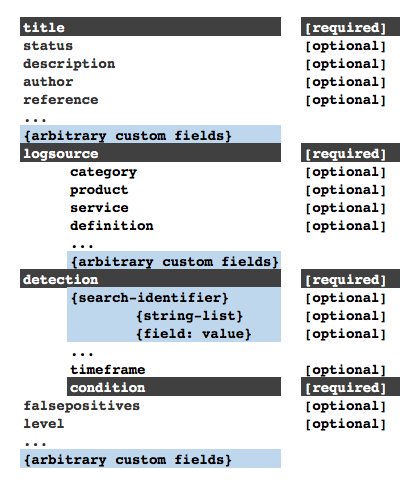
\includegraphics[scale=0.525]{figures/new-rule-format/Sigma_Schema.png}

Image source: \url{https://github.com/Neo23x0/sigma/wiki/Specification}

\section{Event correlation}

Say something about event correlation in general here. Maybe add a overview-figure?

\subsection{Scenario-based Correlation}
\iffalse
https://dl.acm.org/doi/pdf/10.1145/1501434.1501479
\fi
\subsection{Statistical Correlation}
\subsection{Temporal Correlation}
\subsection{Hybrid approaches}

\iffalse
\textcite{Ludovic_2004} to propose a fully functional intrusion detection system based on event and alert correlations. Among the several approaches available in the literature, we chose to implement a language driven signature based correlation. Uses FSM to implement the multi-pattern rule matching detection algorithm.
\fi
\subsection{Finite State Machines}
% What are finite state machines?
A finite-state machine, a system is abstracted into mathematical model which can have exactly one of a finite number of states at a time. A finite-state machine has a fixed set of possible states, a set of inputs that change the state, and a set of possible outputs as described by \textcite{keller_2001}.
The next state of a finite-state machine is based on the current state that the machine is in, and the input that change the state.
There are generally considered to be two kinds of finite-state machines, deterministic finite-state machines and non-deterministic finite-state machines. In a deterministic finite-state machine, every state has only one transition per input, as opposed to the non-deterministic state machine, where an input can lead to none, one or many transitions for a given state. Since the deterministic finite-state machine is a more strict version of the non-deterministic finite-state machine, that leads to that by definition, a deterministic finite-state machine is also a non-deterministic finite-state machine.
For example, assuming that we have the following three events in order:
\begin{enumerate}
    \item the process '$word.exe$' started
    \item the process '$googlechrome.exe$' started
    \item The process '$powershell.exe$' started
\end{enumerate}
If we want to trigger an alert when we see the $word.exe$ process is created, and then the $powershell.exe$ process afterwards, we can design a simple non-deterministic state machine like the one in Figure \ref{fig:finite-state-machine}. When applying the above-mentioned events to this finite state-machine, event number one will move our state from $s_0$ to $s_1$. Event number two will not do any transitions and change the state (one of the benefits of using a non-deterministic state machine). When event number three occurs, the state machine transitions from $s_1$ to $s_2$, and our accepting state is reached, which fulfills the state machine and we can create an alarm.
\begin{figure}[ht]
\centering
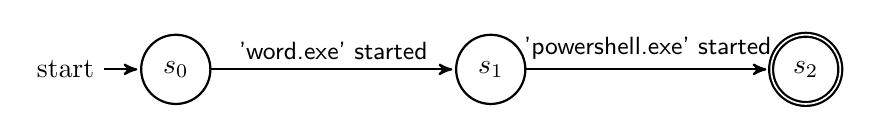
\begin{tikzpicture}[->,>=stealth',shorten >=1pt,auto,node distance=4cm,
                    thick,main node/.style={circle,draw,font=\sffamily\Large\bfseries}]
  \node[initial,state] (p1) {$s_0$};
  \node[state] (p2) [right of=p1] {$s_1$};
  \node[state,accepting] (p3) [right of=p2] {$s_2$};

  \path[every node/.style={font=\sffamily\small}]
    (p1)
        edge node {'word.exe' started} (p2)
    (p2)
        edge node {'powershell.exe' started} (p3)
    ;
\end{tikzpicture}
\caption{Example of non-deterministic finite-state machine}
\label{fig:finite-state-machine}
\end{figure}
One of the benefits of the finite-state model is that it is possible to specify if the order of the events are important or not. If the event order is not of interested, a finite-state machine as shown in Figure \ref{fig:finite-state-machine-2} can represent the same case as seen in Figure \ref{fig:finite-state-machine}.
\begin{figure}[ht]
\centering
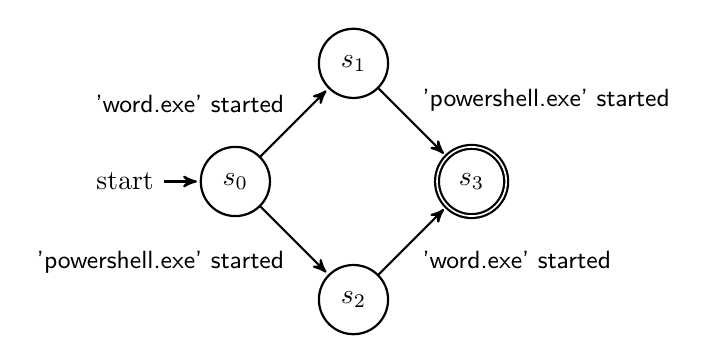
\begin{tikzpicture}[->,>=stealth',shorten >=1pt,auto,node distance=1.5cm,
                    thick,main node/.style={circle,draw,font=\sffamily\Large\bfseries}]
  \node[initial,state] (s0) {$s_0$};
  \node[] (middle) [right of=s0] {};
  \node[state] (s1) [above of=middle] {$s_1$};
  \node[state] (s2) [below of=middle] {$s_2$};
  \node[state,accepting] (s3) [right of=middle] {$s_3$};

  \path[every node/.style={font=\sffamily\small}]
    (s0)
        edge node {'word.exe' started} (s1)
        edge node [swap] {'powershell.exe' started} (s2)
    (s1)
        edge node {'powershell.exe' started} (s3)
    (s2)
        edge node [swap] {'word.exe' started} (s3)
    ;
\end{tikzpicture}
\caption{Example of non-deterministic finite-state machine}
\label{fig:finite-state-machine-2}
\end{figure}

An approach to use finite-state machines for event correlation has been shown by \textcite{Bouloutas_1992}. The authors use observed events that are generated by the monitored process to feed into the modelled finite-state machine that represent the monitored process. If an event arrives that leads to an invalid state in the model, an error is produced.

One of the main drawback with the finite-state machine is the missing notion of time. As shown in Figure \ref{fig:finite-state-machine-2} we can take into account order of events, but a finite-state machine does not separate on the time difference between events that are streamed into the model.

\subsection{Rule-based Event Correlation}

\todo{Give an intro into the world of correlating events, why is it so valuable?}

\begin{itemize}
    \item Reduce alert-fatigue by generating high-fidelity alerts.
    \item Gather up smaller events that in and of them self are not worthy an alarm.
\end{itemize}

Rule-based event correlation software is historically known as a expert system. The work of \textcite{cronk_1988} defines an expert system as a "problem-solving software that embodies specialized knowledge in a narrow task domain to do work usually performed by a trained, skilled human.".

According to \textcite{cronk_1988}, expert systems are organized around three levels; data, control and task knowledge. \todo{See figure 2 in paper. It should be incorporated in some way, as it pretty much defines how we have built MEC}.

Traditionally, creating the rules that goes into a knowledge base is in \textcite{cronk_1988} defined as two-fold; first you have the subject-matter expert which has the expertise and knowledge about which events you are interested in creating correlations against, and secondly the knowledge engineer which is familiar with how the expert system works and how the rules has to be written to be understood by the system.
In more modern settings, usually the subject-matter expert is also able to write rules

What are some of the drawbacks of rule-based event correlation?

\begin{itemize}
    \item Doesn't learn or adapt
    \item Requires the subject-matter expert to define the rules, and the knowledge engineer to implement them
    \item Time-consuming to write and "push" rules into the system
    \item Requires testing and monitoring to make sure that:
    \begin{enumerate}
        \item the rule triggers on the intended events and
        \item the rule does not create tons of alerts that will flood the analysts handling the alerts
    \end{enumerate} 
    \item Maintenance of the rule repository is time-consuming
    \item Networks may differ, so it's not given that a rule that fits into one network, can automatically be used in another.
\end{itemize}

Regardless of all the drawbacks, we see a common trend that rule-based systems are the most common when it comes to network-based monitoring (see Suricata, Snort) as well as for log data in SIEMs like Splunk, ELK, OSSEC and OSSIM.


There exists several different types of software that makes it possible to correlate events in real-time based on log data.

Software based on event correlation commonly referenced in academia today is largely defunct or the source code is unavailable. 

\begin{itemize}
    \item Swatch and 2swatch - defunct, single-threaded. Last updated in 1997?
    \item logsurfer \textcite{thompson_2017} written in C. Improves upon Swatch.
    \item Simple Event Correlator (SEC) is still being actively developed to this date. This is the software that is the most prominent in the literature that I have found. I will address that tool in its own separate section under \ref{sec:SEC}.
    \item Variable Temporal Event Correlator (VTEC) - Built custom for log monitoring and correlation at the company Advanced Micro Devices (AMD). Can not find source code. Feature distributed "workers" and a "variable server" that holds state. Written in Perl and the software uses Perl-based rules.
    \item Event Query Language (EQL). Part of Endgame/Elastic. Written in Python. Scales vertically, same as SEC. Implements a Abstract Syntax Tree for Windows Event Logs specifically.
    \item KSQL - Supports correlation based on time in a Kafka queue. Limited to Kafka as queuing technology.
    \item Splunk - One of the most popular Enterprise SIEM solutions. Supports writing "alerts" that allow time-based correlations.
\end{itemize}
There are several other correlation-based systems other than the ones mentioned above, but they employ some form of machine learning or statistical analysis instead of a rule-based approach. This is usually used for anomaly detection or "finding the unknown" in a dataset, which is not the focus of this thesis.

\subsection{Case-based Reasoning}

In case-based reasoning, a previously experienced problem and its solution is called a case. Case-based reasoning is based on the assumption that we can find a solution for a new problem by finding past cases that are similar, and then reusing the solution to solve the new problem. The reasoning is then further enforced by adding the problem and the solution to the case library for future use as described by \textcite{aamodt_1994}.
As stated by \textcite{slade_1991}, case-based reasoning is similar to how humans approach new problems by assimilating past experiences and adapting them to new situations.

Figure \ref{fig:case-based-reasoning-cycle} describes the cycle used in case-based reasoning from a high-level perspective.
Under each step in the cycle there are multiple tasks that may be necessary to conduct before continuing on with the cycle. For instance, the "Retrieve" step might need to identify which features of the problem to search the Case Library for.
\begin{figure}[ht]
\centering
%\tikzstyle{startstop} = [rectangle, rounded corners, minimum width=3cm, minimum height=1cm,text centered, draw=black, fill=red!30]
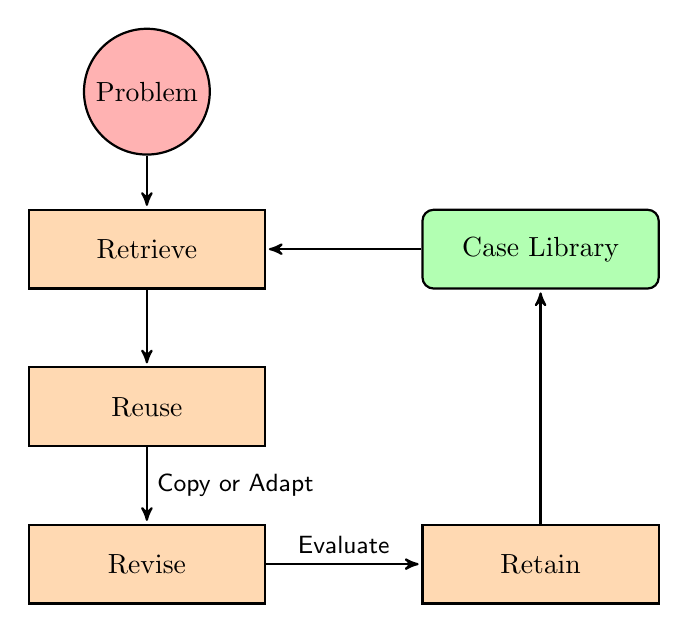
\begin{tikzpicture}[->,>=stealth',shorten >=1pt,auto,node distance=2cm,
                    thick,main node/.style={circle,draw,font=\sffamily\Large\bfseries},
                    problemm/.style={circle, text centered, draw=black, fill=red!30},
                    stepp/.style={rectangle, minimum width=3cm, minimum height=1cm,text centered, draw=black, fill=orange!30},
                    libraryy/.style={rectangle, rounded corners, minimum width=3cm, minimum height=1cm,text centered, draw=black, fill=green!30}]
  \node (Problem) [problemm] {Problem};
  \node (Retrieve) [stepp, below of=Problem] {Retrieve};
  \node (Reuse) [stepp, below of=Retrieve] {Reuse};
  \node (Revise) [stepp, below of=Reuse] {Revise};
  \node (Retain) [stepp, right of=Revise, xshift=3cm] {Retain};
  \node (CaseLibrary) [libraryy, right of=Retrieve, xshift=3cm] {Case Library};
  
  \path[every node/.style={font=\sffamily\small}]
    (Problem)
        edge node {} (Retrieve)
    (Retrieve)
        edge node {} (Reuse)
    (Reuse)
        edge node {Copy or Adapt} (Revise)
    (Revise)
        edge node {Evaluate} (Retain)
    (Retain)
        edge node {} (CaseLibrary)
    (CaseLibrary)
        edge node {} (Retrieve)
    ;
\end{tikzpicture}
\caption{Case-based reasoning cycle}
\label{fig:case-based-reasoning-cycle}
\end{figure}\\
A example where this might be useful is in a Security Operations Center (SOC). A SOC receives a high number of alerts that have to be handled by an analyst to analyse and propose a response to the alert. The response can vary from simply suppressing the alert as a false-positive, sending an e-mail to the client to alert them, or escalating the alarm to the Incident Response team. Case-based reasoning can then be applied to new alerts by first retrieving the most similar alerts previously handled. The information stored in the previous case can then be used to handle the analysis or solution to an alert. The analyst will then revise the proposed solution, and retain the parts that might be useful for resolving similar future alerts. This follows the case-based reasoning cycle proposed in \citetitle{aamodt_1994} by \textcite{aamodt_1994}.

The retrieval step is difficult because we need to find similar cases that offer solutions that are relevant. Cases may contain attributes that are irrelevant, which might not be clear to the automated retrieval process.
An example of this could be the following: Consider that we receive an alert that a malicious file has been detected on a system. We get the IP, hostname, filename and hash of the file as part of the alert. The analyst decides that the file is benign through analysis. This is then stored as a case. If we then receive another similar alert containing yet again an IP, hostname, filename and hash of the file. The filename in this new alert is identical to the one we received earlier, but the hash is different. Using this data, the case-based reasoning engine should not propose a solution based the fact that the filenames are identical, since the file hashes are different, suggesting that the files are not the same.
To solve this, both the work by \textcite{lewis_1993} and \textcite{davies_1987} propose creating "determination rules" or "determinators" that are either compound attributes or a pointer to which attributes to look at in the case.
Additionally, adaptation of the old solutions to the new problem is a difficult task. While manual specification of the solution in the "Revise" step is possible and somewhat required, too much emphasis on manual intervention or adjustments will defeat the purpose of case-based reasoning. This is why according to \textcite{leake_1996} many case-based reasoning systems have adapted the cycle from Retrieve-Reuse-Revise-Retain to a much shorter Retrieve-Propose cycle that completely eliminates the adaptation.

In the paper \citetitle{schwartz_2002}, the authors \textcite{schwartz_2002} used the intrusion detection system Snort as a basis for a new case-based reasoning IDS that uses the Snort rule base as a case library. Snort rules may in general be too specific and fail to detect certain kind of intrusions, but with the case-based reasoning approach, the retrieval step in the cycle will take care of this by finding cases (rules) that are applicable to the network packet even though the vanilla rule would not create an alert on that packet.
\textcite{Kapetanakis_2014} argue that with the digital traces left by an attacker, it is possible to build a profile for that attacker which can be used to assist in future attacks to identify which attacker is attacking. In the paper written by \textcite{han_2016}, the authors implemented a system called "WHAP" which uses case-based reasoning to compare cyber attacks against websites. WHAP builds on a large database of website defacements, which are custom webpages left on the victim server by the attacker to claim credit for a website hack. The system is then able to take new hacked websites as input, and output similar previous cases where it is likely that the website has been hacked by the same attacker. This can be useful for attribution and forensic investigations.

\subsection{Model-based Reasoning}
Model-based reasoning is a expert system where the target is to create a model that can be used to predict the outcome of input event or faults in the system. The idea of modelling the structure and behavior of a system has its roots in the work done by \textcite{davies_1987} where they explore the use of such models in troubleshooting digital electronics.  There are no fixed way for how a system can or should be modelled. The model itself can be created as a logical formalization using pure mathematics, or as a simulated system using for example a game engine. As \textcite{Dodig-Crnkovic2017} highlight in their paper \citetitle{Dodig-Crnkovic2017}, there is an increased interest in automating the creation of the model of a system. This is based on the fact that creating and keeping a model consistent with the system it is supposed to model, is hard.
\textcite{jakobson_1993} discuss model-based reasoning for alarm correlation for fault management in telecommunications networks in their paper \citetitle{jakobson_1993}.


\iffalse


The managed system is modeled
with respect to its event emission behavior (event model). The programmed knowledge somehow
defines events to be related under some temporal or sequential constraints

A description of the 


structure, the topology, connectivity of components
behaviour description,
a set of principles to guide the troubleshooting \textcite{davies_1987}

\fi

In \citetitle{poll_2003} written by \textcite{poll_2003}, a figure similar to \ref{fig:model-based-reasoning-example} is shown. It outlines the process for checking if a modelled system is consistent with the real world system it is supposed to replicate.

\begin{figure}[ht]
\centering
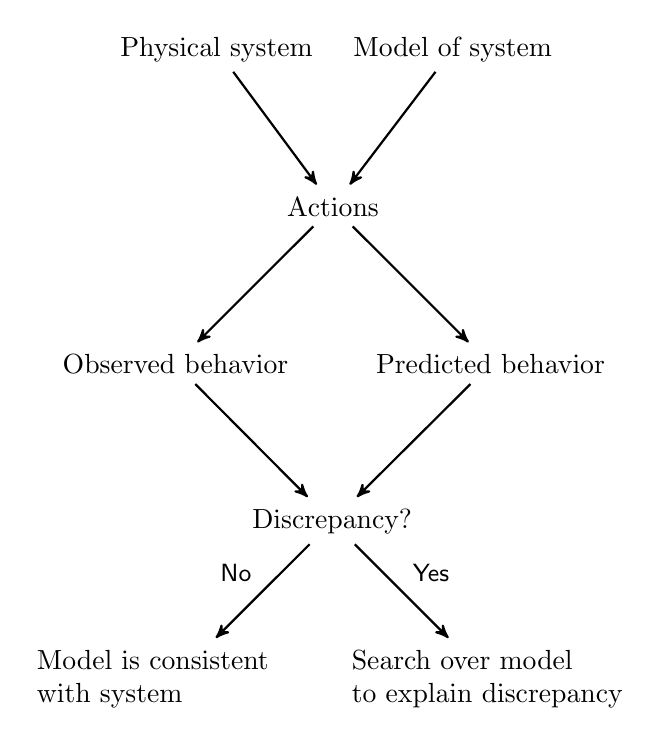
\begin{tikzpicture}[->,>=stealth',shorten >=1pt,auto,node distance=2cm,thick
                    ]
  \node (PhysicalSystem) [xshift=-1cm] {Physical system};
  \node (Model) [xshift=1cm, right of=PhysicalSystem] {Model of system};
  \path (PhysicalSystem) -- (Model) coordinate[midway] (aux);
  
  \node (Actions) [below of= aux] {Actions};
  
  \node (Observed) [below of= Actions,xshift=-2cm] {Observed behavior};
  \node (Predicted) [below of= Actions,xshift=2cm] {Predicted behavior};
  \path (Observed) -- (Predicted) coordinate[midway] (aux2);
  
  \node (Discrepancy) [below of= aux2] {Discrepancy?};
  
  \node (no) [below of= Discrepancy,xshift=-2cm,text width=3.5cm] {Model is consistent with system};
  \node (yes) [below of= Discrepancy,xshift=2cm,text width=3.5cm] {Search over model\\to explain discrepancy};
  
  \path[every node/.style={font=\sffamily\small}]
    (PhysicalSystem)
        edge node {} (Actions)
    (Model)
        edge node {} (Actions)
    (Actions)
        edge node {} (Observed)
        edge node {} (Predicted)
    (Observed)
        edge node {} (Discrepancy)
    (Predicted)
        edge node {} (Discrepancy)
    (Discrepancy)
        edge node [swap] {No} (no)
        edge node {Yes} (yes)
    ;
\end{tikzpicture}
\caption{Illustration of model-based reasoning}
\label{fig:model-based-reasoning-example}
\end{figure}
As stated by \textcite{sethi_2001}, one of the primary drawbacks of model-based reasoning is the requirement to have a well structured system to model and to keep that model updated. Systems that contain fluctuating objects like for example computer networks or network services are not trivial to represent in a formal model. More applicable areas might include hardware diagnostics like shown in the work by \textcite{davies_1987}, or other areas where it is possible to model a more static target system, like for example automobile diagnostics. Finally, in \citetitle{Venkatasubramanian_2003} by \textcite{Venkatasubramanian_2003}, they discuss that various implementations of model-based reasoning is quite computational complex, depending on number of objects in the model and their various inputs and outputs.

\subsection{Codebook-based Event Correlation}
\label{sub:codebook-based-event-correlation}

\begin{figure}[ht]
\centering
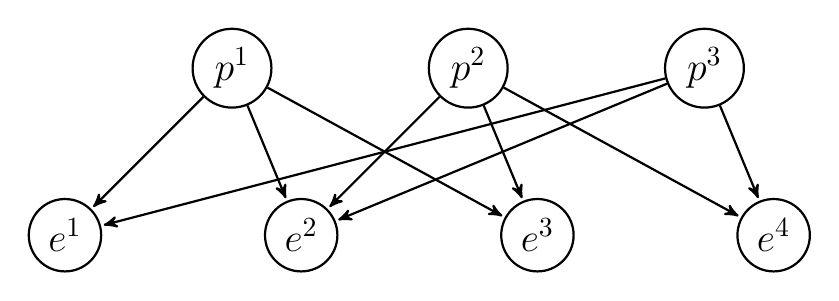
\begin{tikzpicture}[->,>=stealth',shorten >=1pt,auto,node distance=3cm,
                    thick,main node/.style={circle,draw,font=\sffamily\Large\bfseries}]
  \node[main node] (p1) {$p^1$};
  \node[main node] (p2) [right of=p1] {$p^2$};
  \node[main node] (p3) [right of=p2] {$p^3$};
  \node[main node] (e1) [below left of=p1] {$e^1$};
  \node[main node] (e2) [right of=e1] {$e^2$};
  \node[main node] (e3) [right of=e2] {$e^3$};
  \node[main node] (e4) [right of=e3] {$e^4$};

  \path[every node/.style={font=\sffamily\small}]
    (p1)
        edge node {} (e1)
        edge node {} (e2)
        edge node {} (e3)
    (p2)
        edge node {} (e2)
        edge node {} (e3)
        edge node {} (e4)
    (p3)
        edge node {} (e1)
        edge node {} (e2)
        edge node {} (e4)
    ;
\end{tikzpicture}
\caption{Example causality graph used for codebook-based event correlation}
\label{fig:causality-graph-codebook}
\end{figure}

\textcite{yemini_1996} propose that the events caused by problems can be modelled as seen in figure \ref{fig:causality-graph-codebook} where the directed edges of the graph describe the causality of an event. $p^x$ denotes a problem, and $e^x$ denotes an event. To utilize the codebook, each problem node in the graph is converted into a binary vector that can be used to describe its relation to the events on the graph. This is known as a "code". The binary vector contains bits that corresponds to each event in the graph. If a bit is set to a $1$, it indicates that the given problem causes the event that the bit corresponds to. A bit of $0$ indicates that it does not cause the event. These codes then go into the codebook. If we convert the graph in figure \ref{fig:causality-graph-codebook} into a codebook, it will look like table \ref{tab:correlation-matrix}. The graph and codebook needs to be sufficiently large to be able to identify all the problems. If the codebook is too small, it may omit events that are of interest to us. If the codebook is too large, it may contain events that are unnecessarily redundant. One way to approach the problem with codebooks that are too large, is to do what \textcite{yemini_1996} calls "codebook reduction". Codebook reduction is the process of removing events that are "universal" for all problems. In the figure \ref{fig:causality-graph-codebook} and the corresponding table \ref{tab:correlation-matrix} we can see that event $e^2$ is a common event for all the problems. Because of this redundancy, it can be remove to simplify the codebook as show in table \ref{tab:correlation-matrix-reduced}. Further work has been done to enhance the efficiency of the codebook. \textcite{gupta_1999} proposes a two step preprocessing algorithm that ensures mathematical provable codebooks and eliminates events that are unable to distinguish between problems.

When new events occur, the events are converted into a new binary vector. This vector is then compared with the codes in the codebook, and the code that is the most similar is chosen as a means to identify the problem. A simple approach for comparing the binary vectors could be a 1-to-1 comparison to see if the new binary vector exactly matches any of the codes in the codebook, but \textcite{yemini_1996} propose to instead use Hamming distance to calculate the closest match. Using Hamming distance has several benefits, first of all it increases the tolerance for noise or lost events, secondly instead of choosing a single best candidate problem, we can defined a radius that will give us a codebook subset containing possible codes within the given Hamming distance radius.
Because of the novel preprocessing down to binary vectors, codebook-based correlation is faster than other rule-based event correlation techniques. One of the more time-consuming tasks with regard to codebook-based event correlation is the creation of the problems and their mapping to symptom events. The most likely way to produce these codebooks will be as an expert system where a person with deep knowledge about the events in the system are able to map symptoms to problems. In addition, the process of selecting which events might be symptoms of a problem is similar to feature selection in the machine learning landscape. Feature selection is the process of selecting a subset of features that can be used in model construction, which is similar to how the codebook is generated.

One of the biggest limitations regarding codebook-based event correlation is that there is no built-in way to handle time. When a problem has been identified based on a number of symptoms, there is no time window applied, and there is no notion of event order. Furthermore the events do not contain any properties, and would require significant extending to take into account e.g. source hostname, username.

\begin{table}[ht]
\centering
\begin{tabular}{l|llll}
 & $e^1$ & $e^2$ & $e^3$ & $e^4$ \\ \hline
$p^1$ & 1 & 1 & 1 & 0 \\
$p^2$ & 0 & 1 & 1 & 1 \\
$p^3$ & 1 & 1 & 0 & 1
\end{tabular}
\caption{Codebook correlation matrix}
\label{tab:correlation-matrix}
\end{table}

\begin{table}[ht]
\centering
\begin{tabular}{l|lll}
 & $e^1$ & $e^3$ & $e^4$ \\ \hline
$p^1$ & 1 & 1 & 0 \\
$p^2$ & 0 & 1 & 1 \\
$p^3$ & 1 & 0 & 1
\end{tabular}
\caption{Reduced codebook correlation matrix}
\label{tab:correlation-matrix-reduced}
\end{table}

\subsection{Voting approaches}
\subsection{Explicit Fault-localization}
\subsection{Dependency Graphs}


\begin{figure}[ht]
\centering
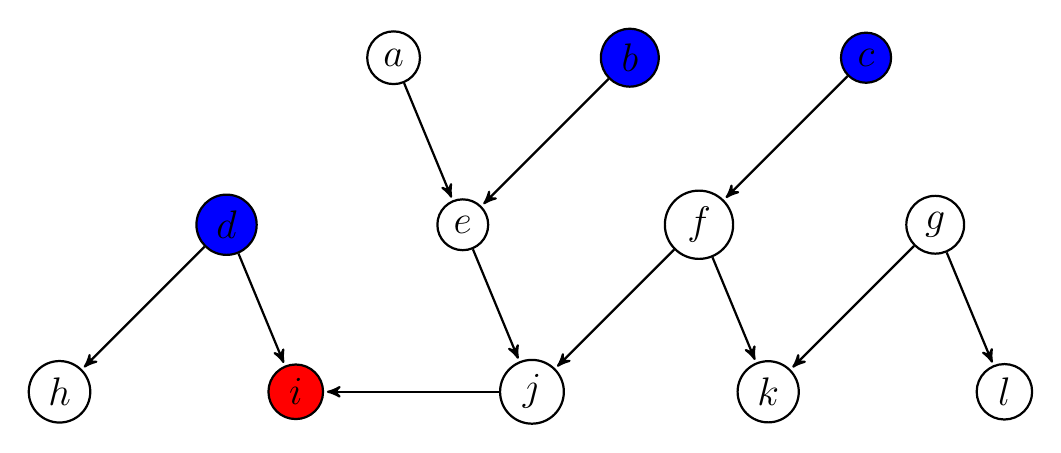
\begin{tikzpicture}[->,>=stealth',shorten >=1pt,auto,node distance=3cm,
                    thick,main node/.style={circle,draw,font=\sffamily\Large\bfseries}]
  \node[main node] (a) {$a$};
  \node[main node,fill=blue] (b) [right of=a] {$b$};
  \node[main node,fill=blue] (c) [right of=b] {$c$};
  \node[main node,fill=blue] (d) [below left of=a] {$d$};
  \node[main node] (e) [right of=d] {$e$};
  \node[main node] (f) [right of=e] {$f$};
  \node[main node] (g) [right of=f] {$g$};
  \node[main node] (h) [below left of=d] {$h$};
  \node[main node,fill=red] (i) [right of=h] {$i$};
  \node[main node] (j) [right of=i] {$j$};
  \node[main node] (k) [right of=j] {$k$};
  \node[main node] (l) [right of=k] {$l$};

  \path[every node/.style={font=\sffamily\small}]
    (a)
        edge node {} (e)
    (b)
        edge node {} (e)
    (c)
        edge node {} (f)
    (d)
        edge node {} (h)
        edge node {} (i)
    (e)
        edge node {} (j)
    (f)
        edge node {} (j)
        edge node {} (k)
    (g)
        edge node {} (k)
        edge node {} (l)
    (j)
        edge node {} (i)
    ;
\end{tikzpicture}
\caption{Example dependency graph}
\label{fig:dependency-graph}
\end{figure}

Similar to the dependency graph used in \ref{sub:codebook-based-event-correlation}, \textcite{Gruschke_1998} suggests that a dependency graph can contain enough information to be used for event correlation, while also being simple to automatically generate. The dependency graph is a directed graph that maps the relationship managed objects. These objects can be hosts in a network, dependencies between software dependencies, and so forth.
In figure \ref{fig:dependency-graph} we have mapped a series of objects as an example. Events are mapped to their corresponding object in the graph (colored in blue, object b, c and d). Then we walk the graph from those objects. As explained by \textcite{Gruschke_1998}, when we optimally find one object node that are common for all the given events, we have most likely found the responsible node. In the example this is marked as red, object i.
\textcite{Gruschke_1998} further outlines that the quality of the root-cause detection can be measured by the depth and length we need to walk the graph at. Objects that are further away from the initial object are less likely to be the root cause, and vica versa.
One of the main drawbacks of dependency-graph-based correlation is the fact that it does not handle multiple, non-related problems very well. \textcite{Gruschke_1998} assumes that only one problem occurs at a time. If multiple problems occur that are not related or affect each other, finding the root-case may prove to be impossible, or select the wrong root-cause object.
Assumes the events are for a single fault. Meaning it will not be able to handle detecting multiple failing nodes.
As with the codebook-based event correlation we discussed in \ref{sub:codebook-based-event-correlation}, dependency graphs also lack the notion of time. Additionally the dependency graph is not taking advantage of attributes on the nodes to further enhance the graph.

\subsection{Bayesian Network-based Event Correlation}

Bayesian networks are one of the most widely used graphical models for representing and reasoning about the probabilistic causal relationships between variables as explained in \textcite{Kavousi_2014}. Bayesian networks are usually represented by directed acyclic graphs. Directed acyclic graphs are finite directed graphs that contain no direct cycles. This means that there is no way to start from a given node, and via the directed edges return back to the same node. Each node in the network represents a variable of interest and the edges describe the relations between these variables.
The Bayesian network is split up into two parts. First there is the graphical model of the network which shows the nodes and the edges that connect them. Secondly, there is the conditional probability tables associated with each node. The table consist of the probabilities that a node is in a given state given the state of its parent nodes.



Both the research done by \textcite{Kavousi_2014} and \textcite{Qin_2004} utilize Bayesian networks to create "Bayesian attack graphs" (BAG) which are models that use Bayesian networks to depict the security attack scenarios in a system.

As a simple experiment using a Bayesian Network for detection, we have the directed acyclic graph as shown in Figure \ref{fig:simple-directed-acyclic-graph}. The nodes are a bit like the ones represented in Codebook-based correlation \ref{sub:codebook-based-event-correlation} where the nodes $B$ and $C$ represent two symptom events that are analyzed by the system, these can be events from an IDS, host machine logs, web logs, et cetera. The node $A$ represent a problem node and is not connected to any specific events. The purpose of this Bayesian network, is to answer the following question: What is the probability that, when we observe the two events $B$ and $C$, we have a problem $A$?

To calculate this, we first need the the conditional probability tables, which are given in Table \ref{tab:probabability-tables}.

\begin{figure}[ht]
\centering
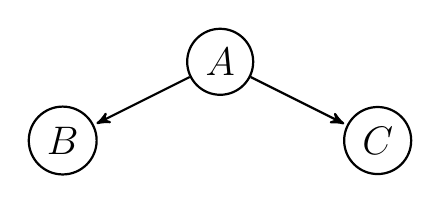
\begin{tikzpicture}[->,>=stealth',shorten >=1pt,auto,node distance=1cm,
                    thick,main node/.style={circle,draw,font=\sffamily\Large\bfseries}]
  \node[main node] (a) {$A$};
  \node[main node] (b) [below of=a,xshift=-2cm] {$B$};
  \node[main node] (c) [below of=a,xshift=2cm] {$C$};

  \path[every node/.style={font=\sffamily\small}]
    (a)
        edge node {} (b)
        edge node {} (c)
    ;
\end{tikzpicture}
\caption{Simple example directed acyclic graph}
\label{fig:simple-directed-acyclic-graph}
\end{figure}

\begin{table}[ht]
\centering
\begin{tabular}{|l|l|}
\hline
$P(A = 0)$ & $P(A = 1)$ \\ \hline
$0.8$ & $0.2$ \\ \hline
\end{tabular}
\begin{tabular}{|l|l|l|}
\hline
$A$ & $P(B = 1|A)$ & $P(B = 0|A)$ \\ \hline
$1$ & $0.9$ & $0.1$ \\ \hline
$0$ & $0.05$ & $0.95$ \\ \hline
\end{tabular}
\centering
\begin{tabular}{|l|l|l|}
\hline
$A$ & $P(C = 1|A)$ & $P(C = 0|A)$ \\ \hline
$1$ & $0.95$ & $0.05$ \\ \hline
$0$ & $0.05$ & $0.95$ \\ \hline
\end{tabular}
\caption{Conditional probability tables}
\label{tab:probabability-tables}
\end{table}

We can then calculate the probability that $A$ has occurred, given that we have observed the events $B$ and $C$ by using Bayes' theorem.
\begin{align*}
    &P(A=1 | B=1, C=1)\\
    &=\frac{P(A=1)P(B=1,C=1|A=1)}{P(B=1,C=1)}\\
    &=\frac{P(A=1)P(B=1,A=1)P(C=1,A=1)}{P(A=1)P(B=1|A=1)P(C=1|A=1)+P(A=0)P(B=1|A=0)P(C=1|A=0)}\\
    &=\frac{0.2\cdot0.9\cdot0.95}{(0.2\cdot0.9\cdot0.95)+(0.8\cdot0.05\cdot0.05)}\\
    &\approx 0.9884
\end{align*}
In this case, we see that there is a 98.8\% chance that the problem/alert $A$ has happened, by observing the arrival of the two events $B$ and $C$.


\subsection{Neural Network Approaches}
\subsection{Etc}


\section{Simple Event Correlator}
\label{sec:SEC}

In the research that I have found, SEC is the most commonly referenced and used software for event correlation across different syslog events. It is widely used, and has been deployed in several different sectors and industries (Finance, Telecom, IT security, Government, Retail, etc. \textcite{vaarandi2005tools}) and utilized for several different purposes like fraud detection, insider-threat detection, system fault and availability and security events. SEC is quite versatile, as it is agnostic to the type of log event that it receives. SEC uses rules that are using Perl-style regular expressions for matching events and extracting data from the event itself using sub-expressions. The extracted data can then be used to correlate between other matching events.

However, even though SEC is popular and commonly used, there are several improvements that could be done. Some of the constraints include:
\begin{itemize}
    \item Heavily based on regular expressions for writing rules, which makes it both hard to analyze rules, modifying existing rules and writing new rules.
    \item Current version can only be scaled vertically. The context-state used for correlation is per-process only and therefore any and all correlation between events have to happen in the same process. It is possible to use SEC in a multi-process fashion to handle separate log types, but this removes the possibility to correlate between those log types. 
    \item Few open source rules and rule-sets. The analyst generally has to start from scratch writing their own rules
    \item Limited support for multi-line logs
    \item Windows Event Logs has to be converted to syslog
    \item Made generic, not specific for Windows Event Logs
\end{itemize}


\subsection{SEC rule format}
\n{Move this section somewhere else}
\begin{lstlisting}
type=single
ptype=regexp
pattern=(\S+)sshd.*
desc=This is a description
\end{lstlisting}

\subsubsection{type}
Type of rule. There are many different types here.
I have focused on rules using "SingleWithThreshold" which takes an action if there are X number of matches in Y time.

Single

Suppress

Calendar

SingleWithSuppress

Pair

PairWithWindow

SingleWith2Thresholds

EventGroup

SingleWithScript

Jump

\subsubsection{ptype}
Pattern type. RegExp is a Perl regular expression. Can use variables.

SubStr

PerlFunc

Cached

TValue

\subsubsection{pattern}
The pattern that the log line will we tested against. The value of this pattern is based on the ptype. For example, if the ptype is set to "RegExp", the pattern will be a Perl regular expression.

\subsubsection{desc}
Description field. But used for defining "scopes" when correlating.

\subsubsection{action}
The action to take when the rule "hits".

\subsubsection{continue}

\subsubsection{context}

\chapter{Methodology}
\label{chap:methodology}

\iffalse
The type of research you did
How you collected your data
How you analyzed your data
Any tools or materials you used in the research
Your rationale for choosing these methods

\begin{enumerate}
    \item What is the state of the art for real time event correlation?
    \item How can we improve the way real time event correlation is done for Windows Event Logs? %How can multi-threaded programming language and better rule formats improve how real time event...
    \item What is the performance of our proposed method, and how does it compare to other methods?
\end{enumerate}

\fi

One of the main goals of this thesis is to explore if there is any way that we can improve the way real time event correlation is done and how our improvement compare to other methods. As outlined in \cref{chap:background} we have chosen to compare our solution against \acrfull{sec}. In addition to the focus towards \acrshort{sec}, we will particularly look at event correlation of Windows Event Logs. In the following chapter we will discuss the methodology used address these goals. We will evaluate which datasets exist and should be used, we will discuss the various ways we can improve how event correlation can be done, and we will take a look at how that performance change can be measured.

\section{Datasets}
\label{sec:datasets}
To properly address the research questions proposed, it is important to have one or more datasets that can be used to evaluate the performance of the proposed solution in this thesis.
There is not a vast variety of available datasets that focus on Windows Event Logs publicly available, but there are some that have surfaced in the recent years. We will present those in the following section and offers a short evaluation in the context of this thesis.

\subsection{Evaluation of existing datasets}
\label{sub:evaluation-of-existing-datasets}
When evaluating which datasets we want to use for our experiments, we first have to define some parameters that we can measure the datasets by:
\begin{itemize}
    \item Size - The dataset must be large enough to measure the performance of existing solutions and our proposed solution.
    \item Representative - The dataset must be representative of the real world
    \item Up to date - The dataset should preferably be of a recent date
\end{itemize}

\subsubsection{Boss of the SOC}
Boss of the SOC (BOTS) are datasets created for Splunks Boss of the SOC capture the flag competitions \cite{bossofthesocdatasets}. The datasets are created in a controlled environment, where some adversarial actions has taken place. The contestants have to analyze and hunt in the data to answer several security-related questions which grant points.

There are currently three different datasets available. Each with a different focus. The first dataset consists primarily of Suricata \cite{Suricata49:online} and Windows events. The second dataset also contains Suricata and Windows events, in addition to more application specific logs like Symantec Endpoint Protection, Weblogic, MySQL etc. The third and last dataset focuses more on cloud and hybrid environments and do not contain the same amount of Windows event logs for instances.

The datasets from BOTS are released in a Splunk pre-indexed format, meaning that one would have to set up a Splunk instance, import the indexed datasets, and then export the datasets out in a more usable format (like JavaScript Object Notation (JSON)). 

\subsubsection{Mordor}
The Mordor datasets \cite{mordor_datasets} are pre-recorded events generated by simulating adversarial techniques in a test environment using common red team tools like Empire and Cobalt Strike.

There currently exists two datasets under the Mordor project, namely APT29 and APT3. These datasets contain Windows event logs from simulated Advanced Persistent Threat (APT) actions. These actions are predefined by the MITRE ATT\&CK Evaluations project \cite{MITREevals}. The MITRE ATT\&CK Evaluations project is created as a way to evaluate different endpoint solutions ability to detect various adversarial techniques, tactics and procedures. The adversarial actions are maps to techniques under 10 categories in the MITREs ATT\&CK Matrix \cite{MITREmatrix}, as shown in \cref{tab:mitre-attack-categories}.

\begin{table}[htbp]
\centering
\begin{tabular}{|l|}
\hline
Categories \\ \hline
Initial Access \\
Execution \\
Persistence \\
Privilege Escalation
Defense Evasion \\
Credential Access
Discovery \\
Lateral Movement \\
Collection \\
Command and Control \\
Exfiltration \\
Impact \\ \hline
\end{tabular}
\caption{List of MITRE ATT\&CK Matrix categories}
\label{tab:mitre-attack-categories}
\end{table}

We will focus on the APT3 dataset. This dataset consists of two subsets, one for each scenario as outlined by MITRE in their Attack Emulation Overview \cite{MITREattackevalapt3} for APT3.

\subsubsection{Synthetic datasets}
Synthetic data is datasets that are generated and design with the intent to measure some specific condition or event that may not be found in real world data, or that the real world data would be hard to come by, as told by \textcite{barse2003synthesizing}. There are multiple reasons why one might consider to use a synthetic dataset, like simulating a large period of time which would be unrealistic to capture in real life, simulating extraordinary events occurring, huge data loads, and so forth. Continuing this section, we will consider three different synthetic datasets that we will be applying during our experiments in \cref{chap:experiments}.

It is worth stressing that the synthetic datasets are used strictly for measuring the performance of the systems in a worst-case/best-case scenario, and the dataset is in itself not representative of a real world scenario.

\textbf{Baseline dataset}\\
This dataset is a dataset with events that are all benign. This dataset is useful for measuring the speed at which the tools process and analyse the events, without triggering any rules.

\textbf{High signal, low noise dataset}\\
If we want to test the maximum event correlation throughput possible, we want to use a dataset that is designed to continuously trigger one or more rules. Given that we want to trigger a rule like the one defined in \cref{sigma-example-rule}, a high signal, low noise dataset could be designed to repeat the same 3 log lines that are enough to trigger the rule. 

\textbf{Low signal, high noise dataset}\\
This is the opposite of the high signal, low noise dataset which contained the necessary log lines to repeatedly trigger a specific rule. This dataset only contains the necessary events to trigger a single rule once, the rest of the events are simply background noise. This is pretty similar to the baseline dataset.


\subsection{Datasets used in this thesis}
\label{sec:datasets-used}

For the experiments conducted in this thesis, Multiple datasets have been chosen:

\begin{itemize}
    \item Mordor dataset (APT3, Scenario 1 and 2)
    \item High signal, low noise dataset
    \item Baseline dataset
\end{itemize}
We chose the Mordor dataset as it is sufficiently large enough, representative and up-to-date. Then we have chosen the baseline and high signal, low noise synthetic datasets as they will be used for baselining and giving us best and worst-case scenarios for performance measuring. We do not use the low signal, high noise dataset, as we consider that almost identical to the baseline dataset.

\section{Improving real time event correlation for Windows Event Logs}
\label{sec:improving-real-time-event-correlation-for-windows-event-logs}

With regards to Research Question 2 in Section \cref{sec:researchquestions}, the question we are trying to answer is if there are ways we can improve how real time event correlation is done. We will discuss multiple approaches to how this can be achieved in the following section.

\subsection{Compiled language vs. interpreted language}
\label{sub:use-compiled-language}


As previously stated in \cref{sec:SEC}, \acrshort{sec} is written in the Perl language. Perl is an interpreted language that according to its creator \textcite{wall1994perl} is "optimized for scanning arbitrary text files, extracting information from those text files, and printing reports based on that information". Being an interpreted language means that the code is not compiled into machine code and executed like a compiled language does, but the interpreter parses the code step-by-step and execute its actions in subroutines. We can see an overview of both in \cref{fig:compiled-and-interpreted-language}.


There are many benefits to choosing a interpreted language. The interpreter can hide a lot of the complexity when programming, which means that a interpreted language can be easier to write, use and understand. Similarly to the benefits seen with the rules in rule-based event correlation \cref{sub:rule-based-event-correlation}, the programming language can be written with a close similarity to the human language. Additionally, the programs can run cross-platform, as the interpreter manages the lower level details of the specific architecture that we are executing code on.

The main disadvantage is the additional overhead required by the interpreter. Compiled code will generally always be faster than interpreted code, because it runs closer to the "bare metal". When we want to increase performance, working with compiled languages are generally considered the right thing to do.

In the compiled language world, C and C++ has been the kings for a long time. In recent years, other languages like Go \cite{golang} and Rust \cite{Rust} has seen the light of day, and are increasing in popularity. Benefits of the new generation of compiled languages is the built in features for memory safety, safe concurrency, security and better designed languages that makes it easier to get started with the language. This has been the main issue with traditional compiled programs, they are harder to write and easier to get wrong than a program written in a interpreted language.

While this section might give the impression that there is a black and white difference between compiled and interpreted languages, that is not technically correct. In modern times, languages such as Lisp and Pascal implement both, and Java and C\# are compiled into an intermediate language (bytecode) which is executed in a virtual machine as described in \textcite{henriques2018performance}

\begin{figure}[htbp]
    \centering
    \begin{subfigure}[b]{.45\textwidth}
        \centering
        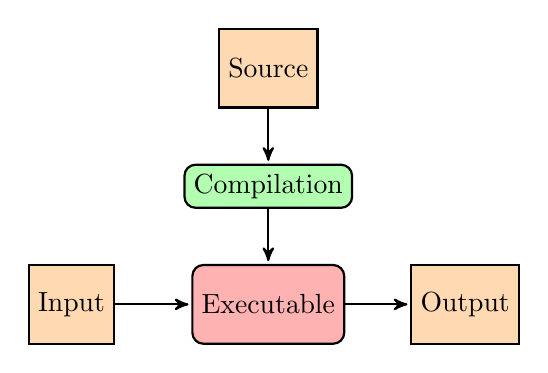
\begin{tikzpicture}[->,>=stealth',shorten >=1pt,auto, node distance=1.5cm, thick,
                    exe/.style={rectangle, minimum width=1cm, minimum height=1cm, rounded corners, text centered, draw=black, fill=red!30},
                    stepp/.style={rectangle, minimum width=1cm, minimum height=1cm,text centered, draw=black, fill=orange!30},
                    libraryy/.style={rectangle, rounded corners, minimum width=1cm, text centered, draw=black, fill=green!30}]
        \node (Source) [stepp] {Source};
        \node (Compilation) [libraryy, below of=Source] {Compilation};
        \node (Executable) [exe, below of=Compilation] {Executable};
        \node (Input) [stepp, left of=Executable, xshift=-1cm] {Input};
        \node (Output) [stepp, right of=Executable, xshift=1cm] {Output};
        
        \path[every node/.style={font=\sffamily\small}]
        (Source)
            edge node {} (Compilation)
        (Compilation)
            edge node {} (Executable)
        (Input)
            edge node {} (Executable)
        (Executable)
            edge node {} (Output)
        ;
        \end{tikzpicture}
        \caption{Compiled language model}
        \label{sfig:compiled-language}
    \end{subfigure}
    \hfill
    \begin{subfigure}[b]{.45\textwidth}
        \centering
        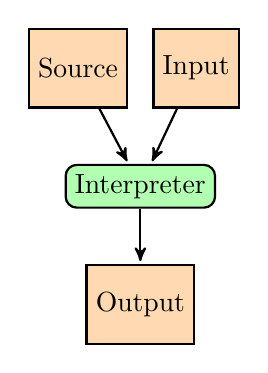
\begin{tikzpicture}[->,>=stealth',shorten >=1pt,auto, node distance=1.5cm, thick,
                    exe/.style={rectangle, minimum width=1cm, minimum height=1cm, rounded corners, text centered, draw=black, fill=red!30},
                    stepp/.style={rectangle, minimum width=1cm, minimum height=1cm,text centered, draw=black, fill=orange!30},
                    libraryy/.style={rectangle, rounded corners, minimum width=1cm, text centered, draw=black, fill=green!30}]
        \node (Source) [stepp] {Source};
        \node (Input) [stepp, right of=Source] {Input};
        \path (Source) -- (Input) coordinate[midway] (aux);
        \node (Interpreter) [libraryy, below of=aux] {Interpreter};
        \node (Output) [stepp, below of=Interpreter] {Output};
        
        \path[every node/.style={font=\sffamily\small}]
        (Source)
            edge node {} (Interpreter)
        (Input)
            edge node {} (Interpreter)
        (Interpreter)
            edge node {} (Output)
        ;
        \end{tikzpicture}
        \caption{Interpreted language model}
        \label{sfig:interpreted-language}
    \end{subfigure}
    \caption{Illustration of compiled vs. interpreted language}
    \label{fig:compiled-and-interpreted-language}
\end{figure}


\subsection{Concurrent execution}
\label{sub:concurrent-execution}

As discussed, \acrshort{sec} is not taking full advantage of the system when only running in a single thread. It is a fair claim that by using multi-threading it is possible to increase the throughput of an alternate solution which will process events much quicker. We can symbolize the difference with the synchronous example in \cref{gantt:synchronous-execution}, and the concurrent process as seen in \cref{sub:concurrent-execution}.

While they both process the same amount of events, the concurrent version handles the total number of events much quicker than the synchronous version. Note that it is not given that each individual event is processed any faster in any of the two examples. In fact, given that we probably want to correlate between the events, the concurrent version could use longer time to handle each event, as it has to check a shared context between the threads, which could cause some overhead.

\begin{figure}[ht]
  \centering
\begin{ganttchart}[
    y unit title = 0.6cm, title height=1,
    vgrid={*1{draw=black!15, line width=.75pt}},
    hgrid,
]{1}{16}
  \gantttitlelist{1,...,16}{1} \\
  \ganttbar[bar/.append style={fill=red!50, rounded corners=3pt}]{Thread 1}{1}{2}
  \ganttbar[bar/.append style={fill=blue, rounded corners=3pt}]{}{3}{4}
  \ganttbar[bar/.append style={fill=red!50, rounded corners=3pt}]{}{5}{6}
  \ganttbar[bar/.append style={fill=blue, rounded corners=3pt}]{}{7}{8}
  \ganttbar[bar/.append style={fill=red!50, rounded corners=3pt}]{}{9}{10}
  \ganttbar[bar/.append style={fill=blue, rounded corners=3pt}]{}{11}{12}
  \ganttbar[bar/.append style={fill=red!50, rounded corners=3pt}]{}{13}{14}
  \ganttbar[bar/.append style={fill=blue, rounded corners=3pt}]{}{15}{16}
\end{ganttchart}
  \caption{Synchronously processing of 8 events}
  \label{gantt:synchronous-execution}
\end{figure}

\begin{figure}[ht]  %t top, b bottom, p page | you can also use h to try to get the figure to appear at the current location
  \centering
\begin{ganttchart}[
    y unit title = 0.6cm, title height=1,
    vgrid={*1{draw=black!15, line width=.75pt}},
    hgrid
]{1}{16}
  \gantttitlelist{1,...,16}{1} \\
  \ganttbar[bar/.append style={fill=red!50, rounded corners=3pt}]{Thread 1}{1}{2}
  \ganttbar[bar/.append style={fill=blue, rounded corners=3pt}]{}{3}{4} \\
  \ganttbar[bar/.append style={fill=blue, rounded corners=3pt}]{Thread 2}{1}{2}
  \ganttbar[bar/.append style={fill=red!50, rounded corners=3pt}]{}{3}{4}\\
  \ganttbar[bar/.append style={fill=red!50, rounded corners=3pt}]{Thread 3}{1}{2}
  \ganttbar[bar/.append style={fill=blue, rounded corners=3pt}]{}{3}{4}\\
  \ganttbar[bar/.append style={fill=blue, rounded corners=3pt}]{Thread 4}{1}{2}
  \ganttbar[bar/.append style={fill=red!50, rounded corners=3pt}]{}{3}{4}
\end{ganttchart}
  \caption{Concurrent processing of 8 events}
  \label{gantt:concurrent-execution}
\end{figure}


\subsection{Better rules}
\label{sub:better-rules}

The rules in the knowledge base is the bread and butter of the rule-based event correlation. And although there are multiple different ways to create rules as discussed in \cref{sec:rules}, it is always worth considering if other rule formats could be more beneficial.
As stated by \textcite{rouillard2004real}, the majority of the computational time used in \acrshort{sec} is spent on matching events against regular expression, so if we could in some way remove the need for the extensive use of regular expressions by using another rule format, that could potentially be a much faster solution.

We outlined a possible rule candidate in \cref{sub:sigma}, namely Sigma. We will look at implementing Sigma when we experiment with the rule change.

\subsection{Proper time management}
\label{sub:time-management}

One of the biggest drawbacks of \acrshort{sec} as outlined in \cref{sec:SEC}, is the fact that when it bases its correlation time on when the event was read from the input file. It does not take into account any timestamps that may be in the logs.
If logs are ingested from multiple systems (like in a enterprise environment) the logs could be delayed for multiple reasons, or if \acrshort{sec} is unable to ingest the log events fast enough (either because of I/O delays or a huge amount of logs), the timestamp of the logs will be different from when the log event was \textit{actually} produced. The consequences of this could be severe, as events that \textit{should} be correlated together in a given timeframe might drift away from each-other and not be correlated at all.

Instead of the time being based on when the event is read, we want to base our correlation on when the event was generated by the source system. Since we are doing the assumption that we will only be working with Windows event logs which have the UTC timestamp in the logs, we are able to use that. However, if we were to expand to ingest other logs as well, we would have to take into account that the time might be represented differently in the log. It is rare to see logs that do not have a timestamp in some form or fashion. The hardest part might be localization, if the timestamp is not written with a specific timezone. However, this will not be a problem in this thesis as all Windows event logs are written with the UTC timezone.

\subsection{Internal representation of logs}
\label{sub:internal-rep-of-logs}
When we are testing the different rules in \acrshort{sec} against a log line, the pattern of the rule is applied against the whole log line. We propose that tokenizing the log before testing each rule could improve the performance.

Tokenizing the log means that we are taking a log in the form of "EventID: 1\\nMachineName: client1\\nUser: john", and parsing it into a object instead, as seen in \cref{example-tokenization}. The benefit of this is that we can query specific parts of the event log directly, instead of having to parse the whole event log every time we want to access a single key-value pair. An example could be if we wanted to access the MachineName or User values from \cref{example-tokenization}, which could do something like this  \lstinline{event['MachineName']} and \lstinline{event['User']}.

\begin{lstlisting}[
    caption={Example tokenization},
    label=example-tokenization,
    language=java]
Object event = {
    EventID = 1
    MachineName = client1
    User = john
}
\end{lstlisting}

Moving away from the large regexes as already discussed in \cref{sub:better-rules} and using tokenization to enable using new rule formats like Sigma could improve the performance of our solution.

\subsection{Support for multiple log formats}
\label{sub:multiple-log-formats}

As briefly discussed in \cref{sub:time-management} the biggest hurdle would be event logs that either do not contain a timestamp, or are syntactically hard to parse or tokenize as discussed in \cref{sub:internal-rep-of-logs}.
In this thesis we are focused on Windows Event Logs, but it is possible that other log sources would be possible to have working without any or little change to the solution this thesis proposes. We consider this future work.

\subsection{Output modularity}
\label{sub:modularity}

Defining different alert output channels. It would be nice to be able to create granular output rules that takes some decision based on the alert severity and sends the alert to the proper channel. Channels could include:

\begin{itemize}
    \item E-Mail
    \item Instant Messaging platforms like Slack, Teams et cetera.
    \item Ticketing system
    \item SIEM products like Splunk
\end{itemize}
We have chosen not to implement these as we focused primarily on performance measurements, and consider this future work.

\subsection{Distributed correlation}
\label{sub:distributed-correlation}

There are multiple reasons why we might consider using a distributed correlation system. A distributed system first of all provides redundancy if one or more ingestion node or correlation server should fail, having the system continue running without experiencing loss in data. This is important because when we are correlating, we never know when a rule might hit, and any loss of data or interruptions in the correlation process can lead to missed alerts. Furthermore, with regard to geolocation, being able to reduce latency by ingesting data from hosts as close to them as possible could improve the real time effectiveness of the system. Any system should be able to handle delayed data, but having as little delay when ingesting data is still preferable. Lastly, if we want to scale up our system to handle bigger loads of data and correlation rules, we need scalability.

As discussed in \cref{sec:SEC}, the authors of \textcite{sec-distributed} considered a few ways to scale \acrshort{sec} as shown in \cref{fig:distributed-sec-concept} and \cref{fig:horizontal-scaling-of-sec}.

When scaling a system, we generally consider two different types of scaling. Horizontal and vertical. Horizontal scaling means that we are adding additional machines into a pool of resources for that particular service. Vertical scaling is adding more power to the existing machine, for instance by increasing the available RAM or upgrading the CPU(s).
There are multiple considerations that have to be done when choosing which way to scale a system. Horizontal scaling usually comes with the drawback of having to manage the pool of resources for each scaled service. Vertical scaling is in general simpler, but at some point it is no longer possible or feasible to scale further with regards to performance and cost.
The implementation show in this thesis is primarily built to scale vertically.
Interesting future work would be to add horizontal scaling to the proposed solution in this thesis, much like in \cref{fig:distributed-sec-concept}, and tackle the challenges associated with load balancing, shared "context memory" between the correlators, and other possible obstacles.

\section{Measuring performance}
\label{sec:measuring-performance}
There are multiple factors that affect the performance of event correlators. All these factors lead to multiple ways that we can measure performance. This section tries to outline the most important ones.

\subsection{Data ingestion speed}
\label{sub:ingestion-speed}

At the start of the data pipeline, we have to ingest our data for processing. Data ingestion is the process of importing data from an external source into our program. The rate at which we are ingesting events are usually measured in events per second.
Data ingestion is based on a emitter sending the data, and a receiver receiving the data. The emitter does not have to be a separate system, it can be a hard disk, RAM or a network-based service. 
The performance related to data ingestion speeds can be bottlenecked by several possible things. The emitter may be bound by the storage medium it is sending data from. If we are reading events from a log file stored to disk, we are bound to the read speed that our disk(s) support. If we are reading events from a process that stores the events in memory, we are bound by the read speeds of our RAM.
With regards to network-based transmission, the choice of transport-layer protocol used can have an impact on transmission speed. Using UDP may be the fastest, but could lead to dropped packages which not optimal. Using TCP ensures that all events are transmitted, but at the cost of additional overhead for re-transmitting lost data, re-arranging packets out of order, et cetera. When transmitting data in a network (both internal and via the internet) encryption is needed to ensure authenticity and tamper protection of the data. But encryption comes at a cost, namely that it takes some time to encrypt and decrypt data when its sent and received.
Additionally, the networking hardware can play a role depending on the setup. The supported speeds of the network card in the emitter and receiver, and any intermediate networking equipment like switches and routers could affect the throughput of events.
There are multiple ways of transmitting data over the network that may affect the ingestion speed, and that is the implementation of how transmitting shall be done. Real-time transmission sends the events as soon as they happen, one-by-one. Another tactic is to use batching or chunking that sends bursts of events instead of sending the events one-by-one. Finally, a hybrid approach is possible where the emitter chooses which type to use depending how many events are being transmitted.
Then we have the ingestion capabilities of the receiver. This boils down to how efficient the receiver is to manage the backlog of events it receives. A simple program might only allow processing one event at the time, blocking incoming new events. A more efficient program might store a backlog of events in RAM, which ensures that it does not block incoming new events.

There are multiple ways we can measure all these different possible bottlenecks. For disk and RAM-based operations we can use profiling tools that come with the operating system to measure the load we are under. We can look at the number and size of the network packages being sent and received. Given an external emitter running for instance the software Kafka, we can get an overview of how fast receivers are fetching data from the emitter. Likewise, we can do the same from the end of the receiver by looking at how many events we are ingesting into our program per second. Finally, we can test the ingestion using timing, by ingesting a set number of events and timing how fast the receiver can ingest them (without any processing other than ingesting), we can calculate the number of events per second.

\subsection{Processing speed}
\label{subs:processing-speed}
Since the ingestion speed discussed in \cref{sub:ingestion-speed} might fluctuate depending on how the data is ingested, measuring the internal processing speed might be more interesting when evaluating the performance of the various solutions. This removes the uncertainties related to ingestion speeds. There are multiple options when looking at internal processing speed. One might look at the processing as a whole from start to finish, or try to separate out the various internal steps that occur during processing. Go features a profiler that will output a graph, showing which functions are taking up the most time during runtime. This can give an idea of where the most of the time is spent during processing.

The processing speed can be affected by several things. First of all the dataset used will matter, as the number of matches will have an effect on the number of alerts generated and contexts updated.
Secondly, the implementation of how rules are processed and checked against events can have a big impact on the processing speed. If the solution is able to quickly disregard events as not interesting, there is a big potential for saving time.
Lastly, the internal handling of contextual information, how that information is accessed and other performance-related improvements all have an effect on the processing speed observed.
% Drawback
The biggest drawback of this approach is the need profiling or timing "inside" the solution. While this might be simple to implement in a new solution, patching such a feature into older solutions can prove to be hard or in the worst case error-prone if the solution being patched is not fully understood.

\subsection{Compound processing speed}
\label{sub:compound-processing-speed}

Measuring the compound processing speed will give us a bird's-eye view of what the total processing speed is. It takes into account both ingestion and processing speeds, measures the total time used, including both I/O and any internal processing.

Depending on the solutions, this might be the best or only option for a good one-to-one comparison between solutions, if they do not support the same ingestion abilities.


\section{Test plan}
As discussed in this chapter we have identified  multiple ways that possibly could improve or further expand the capabilities of existing real time event correlation solutions, more specifically \acrshort{sec}.

In \cref{chap:experiments} we will be using the Mordor \cite{mordor_datasets} APT3 dataset, in addition to three synthetic datasets as explained in \cref{sec:datasets}.

We will focus our experiments around the possible improvements mentioned in this chapter, namely using a compiled language, utilize concurrent execution, test if better internal representation of log data and using other rules might affect performance and lastly implement better time management. Distributed correlation, output modularity and support for multiple log formats is considered future work.
As discussed in \cref{sec:measuring-performance}, there are multiple ways that we can measure the performance of our solution against existing solutions. We will be using compound processing speed as discussed in \cref{sub:compound-processing-speed} for our performance tests.
\chapter{Experiments}
\label{chap:experiments}
The following chapter introduce our improved implementation based on the methodology presented in \cref{chap:methodology}. The software and hardware specifications are listed, the dataset collection and required preprocessing is presented, and we introduce our solution in two step, first a solution that uses the same rule format as \acrshort{sec}, and then a improved version that implements Sigma \cite{Sigma} and a better way for internally representing events as discussed in \cref{sub:internal-rep-of-logs}.

\iffalse
graph the dataset and look at peaks.
Then multiply by potential hosts in enterprise.
Then look at, are we able to handle that amount of events?
What if we use more rules?


The following chapter introduces the actual implementation of the experiment based on the methodology presented in Chapter 4. The collection of the data set, the software versions, the hardware
specifications and the used algorithms during the experiment are presented as well as the experimental design and the technical implementation. It demonstrates the technical execution of the
methodology for reproducibility of the use case.
\fi

\section{Hardware and Software Specifications}
\label{sec:hardwaresoftwarespecs}
The host system used for running the experiments feature a Intel(R) Core(TM) i7-7600U CPU @ 2.80GHz processor and 24 GB memory. The processor features two physical cores, and is capable of running two threads per core. This means that the processor has a maximum of 4 logical cores.

The software versions of interest are:
\begin{itemize}
    \item Ubuntu 18.04.4 LTS, released February 2020
    \item go version go1.13.3 linux/amd64, released October 2019
    \item Perl v5.30.2 built for x86\_64-linux, released March 2020
    \item Simple Event Correlator v2.8.2, released on Jun 2, 2019
\end{itemize}

\section{Dataset preprocessing and analysis}

In total, the two subsets contain 223 563 log lines in JSON format. 116 572 of these are of the type "Microsoft-Windows-Sysmon" which will be the main focus of our experiments.
As previously explained in \cref{sec:SEC}, \acrshort{sec} is created to work with logs that contain one event per line in syslog format. For us to be able to use the Mordor dataset in \acrshort{sec}, we had to convert the \acrshort{json} logs into a syslog-friendly format. We converted the Mordor APT3 datasets by extracting the hostname and the raw Windows Event message which was still intact in the \acrshort{json} events. The script used can be found in \cref{appendix:sysmon-to-syslog-python-script}. 

It was interesting to us to graph the dataset, as a way to identify if the frequency of events are relatively stable, or of there are peaks in the dataset. Using the script found in \cref{appendix:extract-events-in-10s-intervals} we calculated how many events occurred in every 10 second interval in the dataset. This is valuable as it will tell us what the peak number of events might be, and will guide us in understanding if we are reaching our goal of real time event correlation.
In addition, we wanted to look at the number of computers and users in the dataset. This is valuable as it will give us an idea of how large the environment is. We did this using the scripts in \cref{appendix:extract-computers-from-dataset} and \cref{appendix:extract-users-from-dataset} respectively.

\section{Implementation that uses SECs own regex-based rule format}

\subsection{Choosing a compiled language}

As explained in \cref{sub:use-compiled-language}, there are several benefits when using a compiled language in terms of performance gains.

Go \cite{golang} is cross-platform, supports garbage collection, is strongly and statically typed
In addition, Go features powerful built-in profiling tools and race-condition detection that can help development. This is especially valuable as we know we want to implement concurrency, and detecting and fixing any race-condition issues is of great importance.
Go makes building concurrent programs easy by providing features such as Go routines for spawning new threads, and channels for communicating between the threads.


\iffalse
\section{The Go programming language}

This will not be an extensive intro to Go, the interested reader is referred to \textcite{golang} for further details.

\com{Her er en rask intro, argumentasjonen hvorfor vi valgte dette finner du i eksperiment XYZ}
\todo{Why did we choose Go?} \com{Dette er ikke teori/bakgrunn, men mer et metodevalg.}
\subsection{Goroutines}
\todo{What are these lightweight Go threads?}\\
Goroutines are lightweight threads that are handled by the Go runtime.
\subsection{Channels}
The use of channels and goroutines gives us the ability to run in a threaded matter, utilizing multiple cores.
\todo{What are channels? What are some of the considerations we have to take when working with them?}\\
\todo{Are there any best practices?}\\
Channels are the preferred way to communicate between Goroutines in Go.

\subsection{Concurrency vs parallelism}
\todo{Discuss why Go is concurrent, but not parallel}
\fi


Other than the fact that Go is a compiled language and Perl is a interpreted language, the main additions in our implementation is that our version:
\begin{itemize}
    \item Uses Go channels for re-injecting events into the context engine.
    \item 
\end{itemize}

\subsubsection{Workers}


\subsection{Implementation}
When considering which features we wanted to implement from \acrshort{sec}, we chose to implement the features that we saw the best value in. We chose to only implement the \textit{Single} and \textit{SingleWithTreshold} type, and the \textit{RegExp} pattern type. These are the features required to implement the rule found in \cref{sec-example-rule}, and also some of the most popular features observed from the \acrshort{sec} rule repository \cite{sec-rulesets}.

Furthermore, we implemented threading by using Go routines and channels. The architecture can be seen from the \cref{fig:reimplementation-architecture}. While it might seem complex, in reality it is pretty simple. Each block is a separate Go routine running in a lightweight thread. \lstinline{getEvents()} reads events from input, and sends each event on a channel named \lstinline{eventChannel}. The \lstinline{handleEvent()} Go routines (named workers in our implementation), listens to this channel and when a new event arrives, picks it off the channel and starts processing it. As can be seen from \cref{fig:reimplementation-architecture}, the workers are sharing context, that they will lock on if any rules are matching and they need to do some correlation. If a rule matches and issues a \textit{event} action (as shown in \cref{sec-example-rule}), the worker will push the event action on to a new channel that is being listened to by \lstinline{reinjectEvents()}. \lstinline{reinjectEvents()} is a Go routine with the sole purpose to collect events from multiple workers and forward them on a single channel, reinjecting into \lstinline{eventChannel}. This makes the new events available to the the workers, so that they can process the new events. If any of the \lstinline{handleEvent()} workers completes a correlation according to the rule, and the rule issues a \textit{write} action, the action is written to output.

\begin{figure}[htbp]
\centering
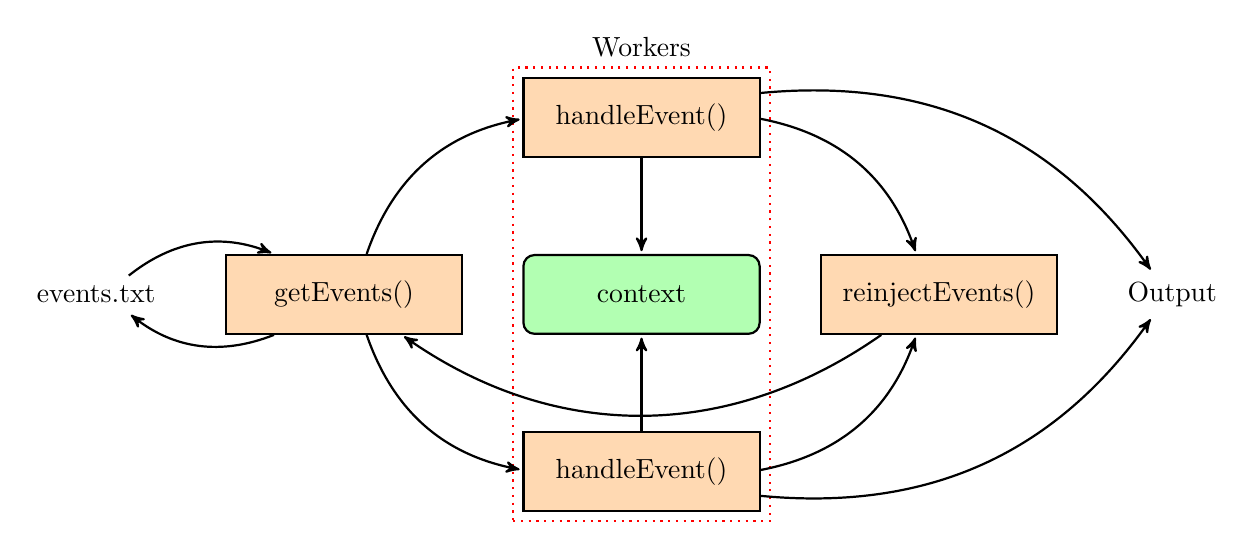
\begin{tikzpicture}[->,
>=stealth',
shorten >=1pt,
thick,
node distance=2.25cm and 0.75cm, % y and x
stepp/.style={rectangle, minimum width=3cm, minimum height=1cm, text centered, draw=black, fill=orange!30},
libraryy/.style={rectangle, rounded corners, minimum width=3cm, minimum height=1cm,text centered, draw=black, fill=green!30},
]
  \node (events) [] {events.txt};
  \node (getEvents) [stepp, right= of events] {getEvents()};
  \node (context) [libraryy, right= of getEvents] {context};
  \node (handleEvent1) [stepp, above of=context] {handleEvent()};
  \node (handleEvent2) [stepp, below of=context] {handleEvent()};
  \node (reinjectEvents) [stepp, right= of context] {reinjectEvents()};
  \node (output) [right= of reinjectEvents] {Output};
  \node[draw=red,dotted,fit=(handleEvent1) (handleEvent2), label={above:{Workers}}] {};
  
  \path[every node/.style={font=\sffamily\small}]
    (events)
        edge[bend left] node {} (getEvents)
    (getEvents)
        edge[bend left] node {} (events)
        edge[bend left] node {} (handleEvent1)
        edge[bend right] node {} (handleEvent2)
    (handleEvent1)
        edge node {} (context)
        edge[bend left] node {} (reinjectEvents)
        edge[bend left] node {} (output)
    (handleEvent2)
        edge node {} (context)
        edge[bend right] node {} (reinjectEvents)
        edge[bend right] node {} (output)
    (reinjectEvents)
        edge[bend left=35] node {} (getEvents)
    ;
\end{tikzpicture}
\caption{Reimplementation in Go}
\label{fig:reimplementation-architecture}
\end{figure}


\section{Implemented a new rule format}
This format relies less on the extensive use of Regexes \com{Hvorfor er dette en fordel? Hvorfor er dette valget smart? Beskriv dette i experiment delen?}, as we saw in the rules used by Simple Event Correlator. \todo{Elaborate on this}
\\
For each log line/event we:

\begin{enumerate}
    \item Tokenize the event into a Event struct. \com{Hva er dette?... Flytt beskrivelsen opp til Experiment i stedet?}
    \item Iterate over every rule, checking if the Event matches the detection-part of the rule.
    \begin{itemize}
        \item If there is a match, we run the Event through the context engine, to see if the conditions are met for the rule.
    \end{itemize}
\end{enumerate}

When we tokenize the event, we take a single line of log/event, and split it into its key-value representation. For instance, the following event log is a single line of text:
\begin{lstlisting}[breaklines=true]
<14>Feb 18 02:29:49 Client02.mrtn.lab Microsoft-Windows-Sysmon[2092]: Process Create:  RuleName:   UtcTime: 2020-02-18 10:29:49.839  ProcessGuid: {dadb16ad-bc9d-5e4b-0000-0010c8fd3600}  ProcessId: 1040  Image: C:\Windows\System32\whoami.exe  FileVersion: 10.0.17763.1 (WinBuild.160101.0800)  Description: whoami - displays logged on user information  Product: Microsoft Windows Operating System  Company: Microsoft Corporation  OriginalFileName: whoami.exe  CommandLine: whoami  CurrentDirectory: C:\Users\mrtn\  User: MRTNLAB\mrtn  LogonGuid: {dadb16ad-2c2d-5e17-0000-0020fc3c1b00}  LogonId: 0x1B3CFC  TerminalSessionId: 1  IntegrityLevel: Medium  Hashes: MD5=43C2D3293AD939241DF61B3630A9D3B6,SHA256=1D5491E3C468EE4B4EF6EDFF4BBC7D06EE83180F6F0B1576763EA2EFE049493A,IMPHASH=7FF0758B766F747CE57DFAC70743FB88  ParentProcessGuid: {dadb16ad-2cf1-5e17-0000-001027122b00}  ParentProcessId: 2748  ParentImage: C:\Users\mrtn\test.exe  ParentCommandLine: .\test.exe
\end{lstlisting}
But after tokenization, it looks like this:
\begin{lstlisting}[breaklines=true]
MachineName: Client02.mrtn.lab
ProcessType: Process Create: 
RuleName:   
UtcTime: 2020-02-18 10:29:49.839
ProcessGuid: {dadb16ad-bc9d-5e4b-0000-0010c8fd3600}
ProcessId: 1040
Image: C:\Windows\System32\whoami.exe
FileVersion: 10.0.17763.1 (WinBuild.160101.0800)
Description: whoami - displays logged on user information  Product: Microsoft Windows Operating System
Company: Microsoft Corporation 
OriginalFileName: whoami.exe
CommandLine: whoami
CurrentDirectory: C:\Users\mrtn\
User: MRTNLAB\mrtn
LogonGuid: {dadb16ad-2c2d-5e17-0000-0020fc3c1b00}
LogonId: 0x1B3CFC
TerminalSessionId: 1
IntegrityLevel: Medium
Hashes: MD5=43C2D3293AD939241DF61B3630A9D3B6,SHA256=1D5491E3C468EE4B4EF6EDFF4BBC7D06EE83180F6F0B1576763EA2EFE049493A,IMPHASH=7FF0758B766F747CE57DFAC70743FB88
ParentProcessGuid: {dadb16ad-2cf1-5e17-0000-001027122b00}
ParentProcessId: 2748
ParentImage: C:\Users\mrtn\test.exe
ParentCommandLine: .\test.exe
\end{lstlisting}
The tokenized version of the event log is stored as a Go struct, which makes it simpler to query specific parts of the event log directly, instead of having to parse the whole event log every time we want to access a single key-value pair. An example would be if we wanted to access the MachineName or CommandLine values from the above example, which would be done like this:  \lstinline{event['MachineName']} and \lstinline{event['CommandLine']}.


\subsection{Context}
\n{What is context?}
\\
When we want to do correlation between two or more events based on a rule, we need to have some kind of overview of what state our rule is in. When a new event arrives that triggers our rule, we need to know if this is the first event, if there are other events that have triggered before it, and most importantly, if the previous events that triggered the rule is within the given time frame of the rule. This is what we call "context".

\subsection{The Context Engine}
One of the benefits of our new implementation is the ability to process events concurrently. But when working with a context that is accessed by several workers concurrently, data races may appear. A data race occurs when two goroutines concurrently accesses the same variable (in this case the context variable), and at least one of the goroutines writes to the variable. The danger here is that we could have two or more goroutines with their own versions of the context that are out of sync. This could lead to data loss and/or a failure to detect when a rule-condition is met. The standard way of dealing with data races like this is to use a mutex. A mutex provides a locking mechanism to ensure that only one goroutine can manipulate a variable at a time.

In our implementation we have integrated a mutex in two different ways, using a shared context mutex and using a rule-based context mutex. \com{Det er ikke så interessant at vi har brukt to forskjellige, men hva oppnår vi? Hva var hensikten med dette?}

\subsubsection{Shared context}

For the shared context, we have a large map that looks like this:
\begin{lstlisting}
context := map[string]{
    Events  []Event
}
\end{lstlisting}
We access it by doing:
\begin{lstlisting}
c := context["CONTEXT_FOR_RULE_1"]
\end{lstlisting}
the variable \lstinline{c} now contain an array of \lstinline{event}s, if there are any for the given key \lstinline{CONTEXT_FOR_RULE_1}. In our implementation we use the ID of the rule for this lookup, as it is an (Universally unique identifier) UUID4-string, and is safe to use as a unique identifier.


Since we may both read and write to the \lstinline{c} variable, we need to lock a mutex for the \lstinline{context} map. We can do this like this:

\begin{lstlisting}
context := map[string]{
    Events  []Event
}
contextMutex := &sync.RWMutex{}

contextMutex.Lock()
c := context["CONTEXT_FOR_RULE_1"]

// Add or remove events to the context here

context["CONTEXT_FOR_RULE_1"] = c

contextMutex.Unlock()
\end{lstlisting}

We now have a goroutine-safe way of accessing and editing our context. The drawback of this is in the design, when multiple goroutines try to access the context, they will have to wait for their turn to lock on the context.

\subsubsection{Rule-based context}
For the rule-based context, both the context and the context mutex is defined in the rule struct itself:
\begin{lstlisting}
type context struct {
    events []event
}

type Rule struct {
	Context        context
	ContextMutex   sync.RWMutex
	Title          string
	ID             string
	...
}
\end{lstlisting}
Accessing and modifying the rule context is pretty similar to the shared context mutex, but instead of the shared context, we are accessing \lstinline{rule} instead:
\begin{lstlisting}
rule.ContextMutex.Lock()
c := rule.Context

// Add or remove events to the context here

rule.Context = c

rule.ContextMutex.Unlock()
\end{lstlisting}


The benefit to doing it this way is clear. If several goroutines are accessing the context at the same time, but are interested in different rules, we will lock on the individual rule mutex instead of a single shared mutex.

There may still be cases when multiple goroutines try to lock on the same rule and have to wait in line. So depending on the number of rules and how often the rules are triggered we may see performance equal to the shared context as a worst case scenario.
\chapter{Results}
\label{chap:results}
In this chapter the results of both experiments, introduced in Chapter \cref{chap:experiments}, are presented and analysed.

\section{Implementation that uses Simple Event Correlators own rule format (regex based)}

\begin{figure}[ht]
\centering
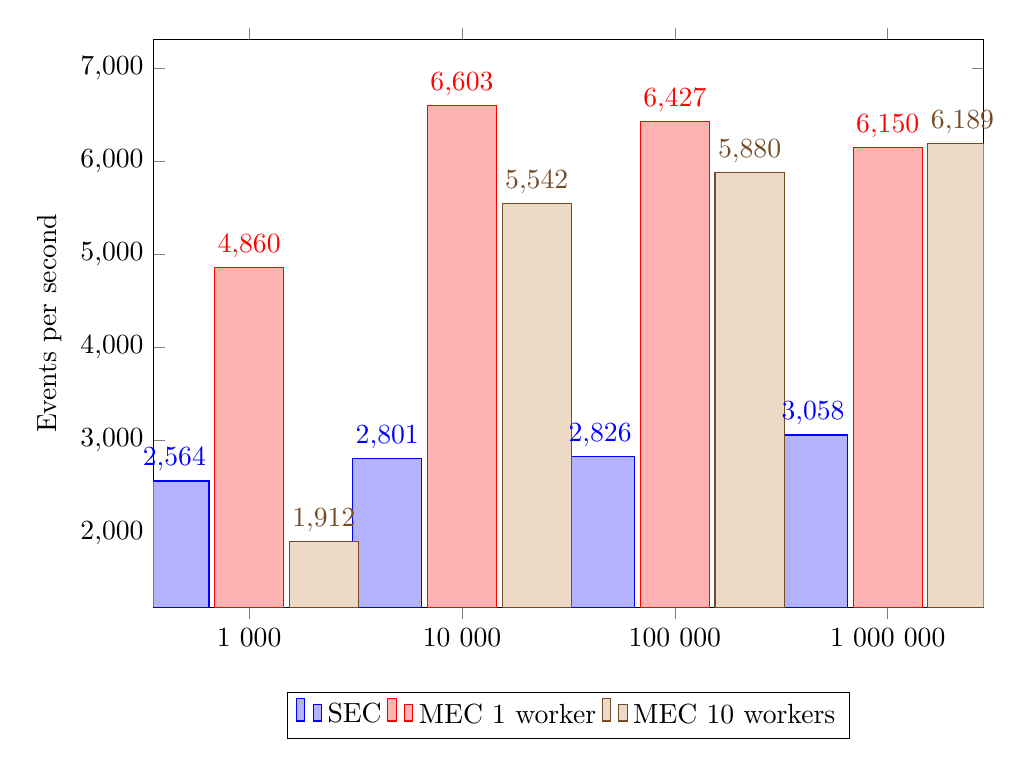
\begin{tikzpicture}
\begin{axis}[
    xtick=data,
	height=250pt,
	ylabel=Events per second,
	enlargelimits=0.15,
	legend style={at={(0.5,-0.15)},
	anchor=north,legend columns=-1},
	ybar,
	bar width=25pt,
	symbolic x coords={1 000, 10 000, 100 000, 1 000 000},
	nodes near coords,
	nodes near coords style={above}
]
\addplot coordinates {(1 000,2564) (10 000,2801) (100 000,2826) (1 000 000,3058)}; % SEC
\addplot coordinates {(1 000,4860) (10 000,6603) (100 000,6427) (1 000 000,6150)}; % MEC1W
\addplot coordinates {(1 000,1912) (10 000,5542) (100 000,5880) (1 000 000,6189)}; % MEC10W
\legend{SEC, MEC 1 worker, MEC 10 workers}
\end{axis}
\end{tikzpicture}
\caption{Baseline dataset}
\label{fig:baseline-perf}
\end{figure}


\begin{figure}[ht]
\centering
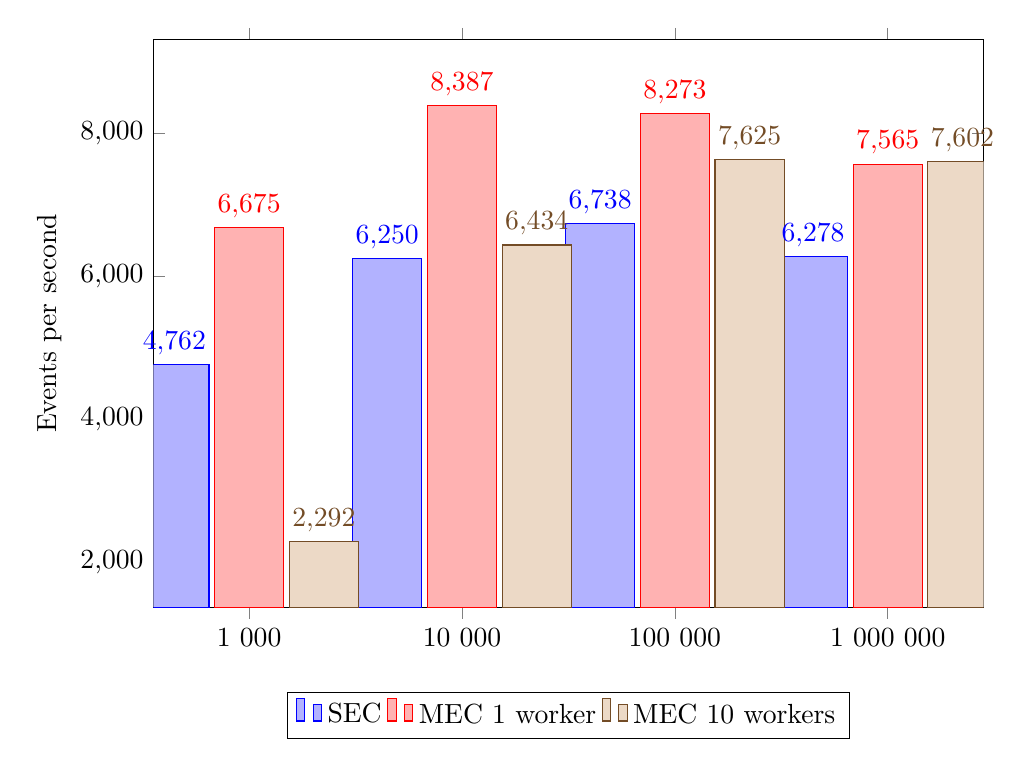
\begin{tikzpicture}
\begin{axis}[
    xtick=data,
	height=250pt,
	ylabel=Events per second,
	enlargelimits=0.15,
	legend style={at={(0.5,-0.15)},
	anchor=north,legend columns=-1},
	ybar,
	bar width=25pt,
	symbolic x coords={1 000, 10 000, 100 000, 1 000 000},
	nodes near coords,
	nodes near coords style={above}
]
\addplot coordinates {(1 000,4762) (10 000,6250) (100 000,6738) (1 000 000,6278)}; % SEC
\addplot coordinates {(1 000,6675) (10 000,8387) (100 000,8273) (1 000 000,7565)}; % MEC1W
\addplot coordinates {(1 000,2292) (10 000,6434) (100 000,7625) (1 000 000,7602)}; % MEC10W
\legend{SEC, MEC 1 worker, MEC 10 workers}
\end{axis}
\end{tikzpicture}
\caption{High signal low noise dataset}
\label{fig:high-signal-low-noise}
\end{figure}


\begin{figure}[ht]
\centering
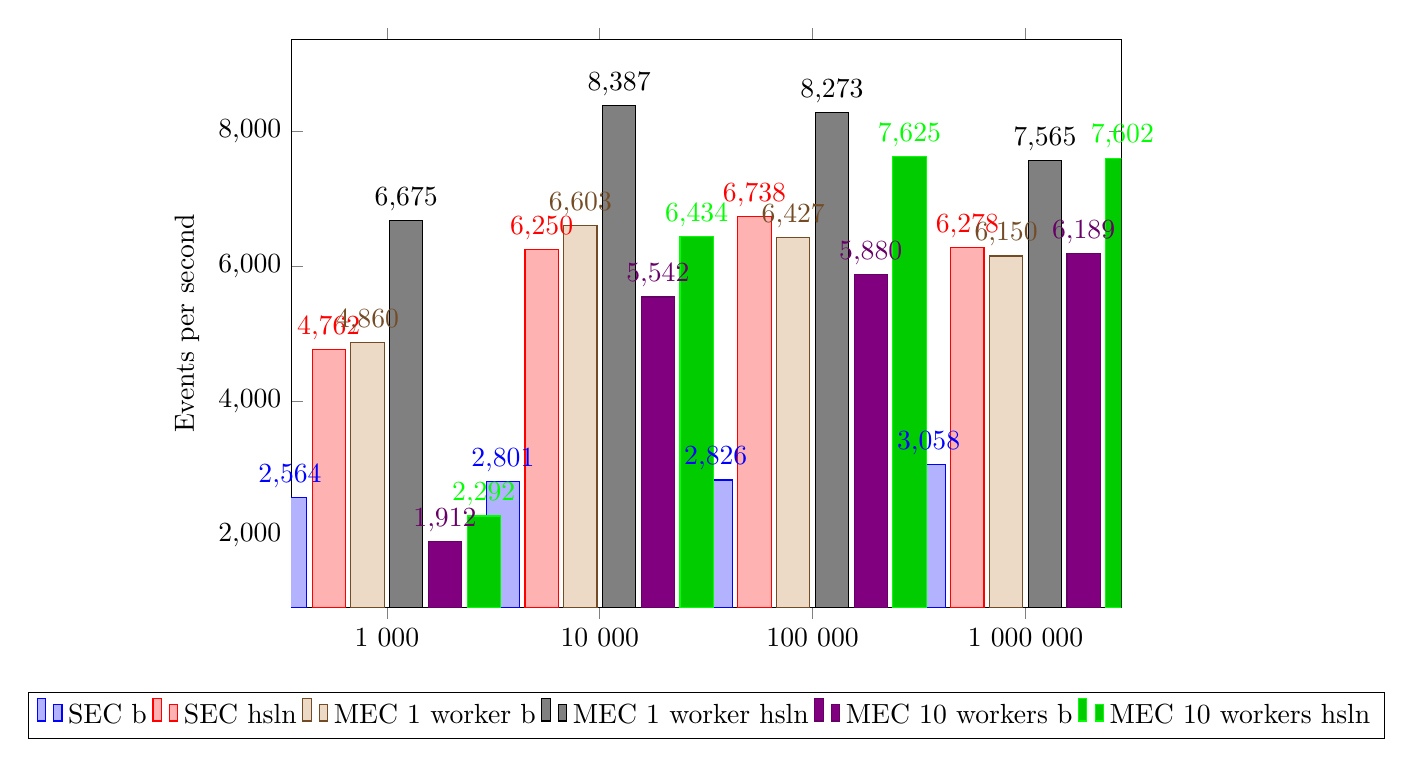
\begin{tikzpicture}
\begin{axis}[
    xtick=data,
	height=250pt,
	ylabel=Events per second,
	enlargelimits=0.15,
	legend style={at={(0.5,-0.15)},
	anchor=north,legend columns=-1},
	ybar,
	bar width=12pt,
	symbolic x coords={1 000, 10 000, 100 000, 1 000 000},
	nodes near coords,
	nodes near coords style={above}
]
\addplot coordinates {(1 000,2564) (10 000,2801) (100 000,2826) (1 000 000,3058)}; % SEC baseline
\addplot coordinates {(1 000,4762) (10 000,6250) (100 000,6738) (1 000 000,6278)}; % SEC high signal low noise

\addplot coordinates {(1 000,4860) (10 000,6603) (100 000,6427) (1 000 000,6150)}; % MEC1W baseline
\addplot coordinates {(1 000,6675) (10 000,8387) (100 000,8273) (1 000 000,7565)}; % MEC1W high signal low noise

\addplot coordinates {(1 000,1912) (10 000,5542) (100 000,5880) (1 000 000,6189)}; % MEC10W baseline
\addplot coordinates {(1 000,2292) (10 000,6434) (100 000,7625) (1 000 000,7602)}; % MEC10W high signal low noise

\legend{SEC b, SEC hsln, MEC 1 worker b, MEC 1 worker hsln, MEC 10 workers b, MEC 10 workers hsln}
\end{axis}
\end{tikzpicture}
\caption{Comparing baseline (b) and High signal low noise (hsln) dataset}
\label{fig:comparing-perf}
\end{figure}

\subsection{Results}
We want to see if our Go implementation can out-perform SEC when handling a high signal, low noise dataset. The Figures \cref{fig:high-signal-low-noise}, \cref{fig:baseline-perf} and \cref{fig:comparing-perf} shows the results for that:
\\
These tests are run with 1 logical core on a "Intel(R) Core(TM) i7-7600U CPU @ 2.80GHz" (2 cores x 2 threads per core = max 4 logical cores) and 24GB RAM.\\
\textbf{What can we say about the performance difference between the two datasets?}\\
It's because of the implementation in SEC and MEC, if we match a rule quickly, we don't have to check all the other rules for a match, and this saves time.\\
\textbf{Why is the MEC10W slower in the start?}\\
Since MEC10W launches ten workers using Go routines, the additional overhead involved with that process is slowing down the performance if you compare it with "single-worker"-style implementations like SEC or MEC with 1 worker.\\
\textbf{Why are the runs on the 1 000 dataset generally lower?}
Because of the small dataset used (1 000), the time spent on general initialization is spread across a lot fewer events, which decreases the events/second throughput.

\subsubsection{Multiple cores}

By using all CPU cores available (4) instead of a single one, we can take better advantage of Gos concurrency model, and raise the throughput when using multiple workers and CPUs as seen in Figure \cref{fig:multicore-hsln-perf} and \cref{fig:multicore-b-perf}.\\
\textbf{What can we say about 1CPU,10W "catching up" to the others around 100 000 events?}\\
This is pretty much the same as what we saw in the single core test.\n{ref her}. The time used to spin up the 10 workers (Go routines) is only outweighed at approximately 100 000 events. This is also why we are seeing a dip when using a dataset of 1 000 events.\\
\textbf{Why are the results of 1CPU,1W, 1CPU,10W and 10CPU,1W generally the same?}\\
This is because they in general are the same. When we are limiting our script to 1 worker, it doesn't really matter how many cores we use, as only one core will be running the worker regardless. There is however a slight benefit to the 4CPU,10W which we can clearly see from the Figure at 1 000 events. The main-function in Go is itself a Go routine, so when we are creating a worker in another core, the main-function can work uninterrupted with reading the log files, while the worker is not blocking since it is running in another core.

\begin{figure}[ht]
\centering
\pgfplotsset{scaled y ticks=false}
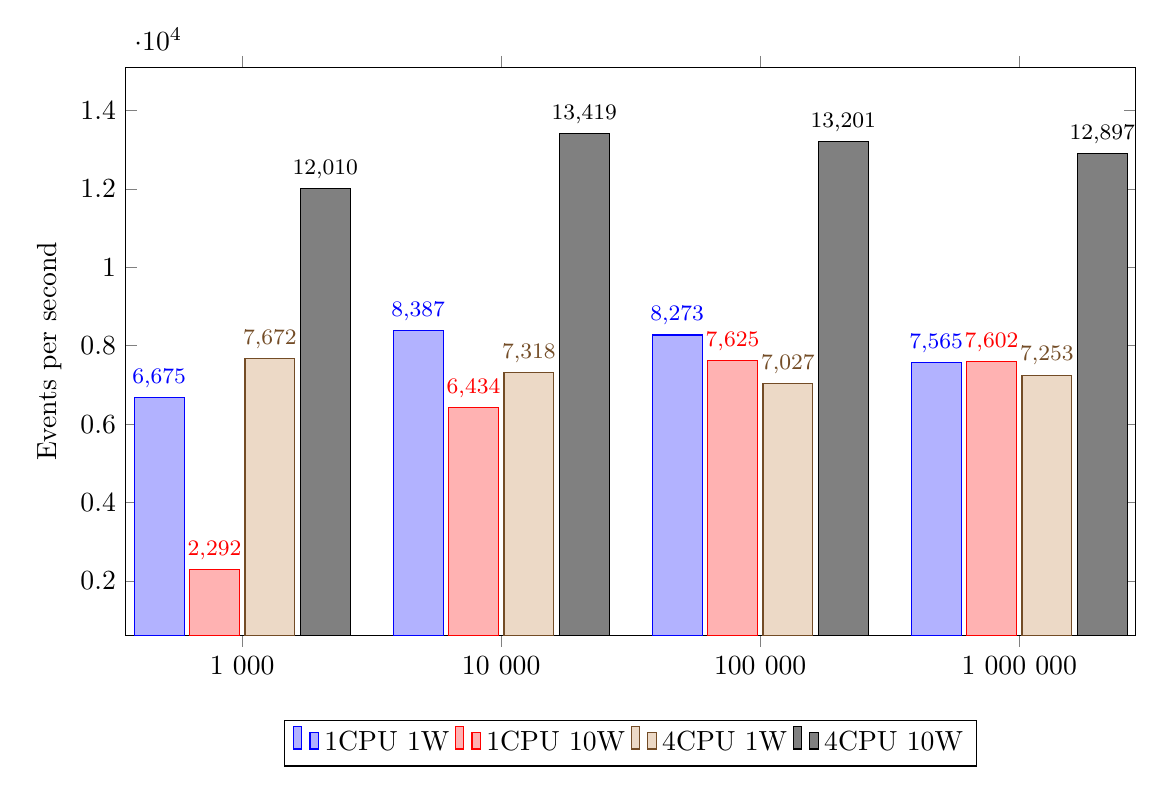
\begin{tikzpicture}
\begin{axis}[
    xtick=data,
    width=410pt,
	height=250pt,
	ylabel=Events per second,
	enlargelimits=0.15,
	legend style={at={(0.5,-0.15)},
	anchor=north,legend columns=-1},
	ybar,
	bar width=18pt,
	symbolic x coords={1 000, 10 000, 100 000, 1 000 000},
	nodes near coords,
	nodes near coords style={above, font=\footnotesize},
]
\addplot coordinates {(1 000,6675) (10 000,8387) (100 000,8273) (1 000 000,7565)}; % 1CPU 1W
\addplot coordinates {(1 000,2292) (10 000,6434) (100 000,7625) (1 000 000,7602)}; % 1CPU 10W
\addplot coordinates {(1 000,7672) (10 000,7318) (100 000,7027) (1 000 000,7253)}; % 4CPU 1W
\addplot coordinates {(1 000,12010) (10 000,13419) (100 000,13201) (1 000 000,12897)}; % 4CPU 10W
\legend{1CPU 1W , 1CPU 10W , 4CPU 1W , 4CPU 10W}
\end{axis}
\end{tikzpicture}
\caption{Concurrency with high signal low noise dataset}
\label{fig:multicore-hsln-perf}
\end{figure}

\begin{figure}[ht]
\centering
\pgfplotsset{scaled y ticks=false}
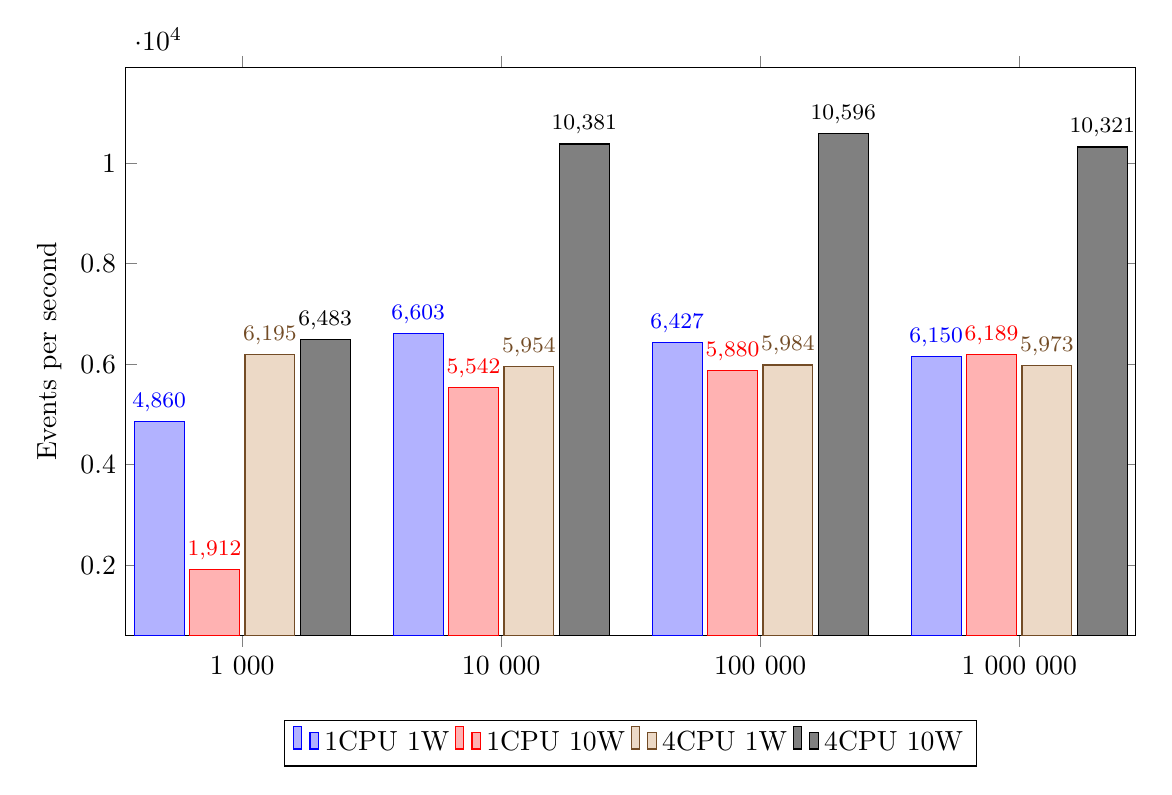
\begin{tikzpicture}
\begin{axis}[
    xtick=data,
    width=410pt,
	height=250pt,
	ylabel=Events per second,
	enlargelimits=0.15,
	legend style={at={(0.5,-0.15)},
	anchor=north,legend columns=-1},
	ybar,
	bar width=18pt,
	symbolic x coords={1 000, 10 000, 100 000, 1 000 000},
	nodes near coords,
	nodes near coords style={above, font=\footnotesize},
]
\addplot coordinates {(1 000,4860) (10 000,6603) (100 000,6427) (1 000 000,6150)}; % 1CPU 1W
\addplot coordinates {(1 000,1912) (10 000,5542) (100 000,5880) (1 000 000,6189)}; % 1CPU 10W
\addplot coordinates {(1 000,6195) (10 000,5954) (100 000,5984) (1 000 000,5973)}; % 4CPU 1W
\addplot coordinates {(1 000,6483) (10 000,10381) (100 000,10596) (1 000 000,10321)}; % 4CPU 10W
\legend{1CPU 1W , 1CPU 10W , 4CPU 1W , 4CPU 10W}
\end{axis}
\end{tikzpicture}
\caption{Concurrency with baseline dataset}
\label{fig:multicore-b-perf}
\end{figure}

\section{Implemented a new rule format}
\subsection{Results}
We are interested in seeing if there are any performance benefits from running our new rule implementation versus the re-implementation of the SEC rules. In the following graph we are running with only a single rule, using our high signal, low noise dataset. The bars labeled "SEC" are our re-implementation of the regular expression-based rules. "Original SEC" is Simple Event Correlator. "MEC" is our implementation with the new rule format.

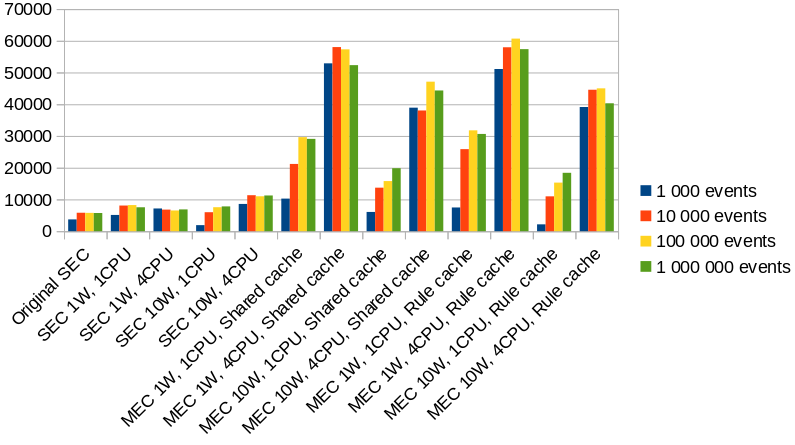
\includegraphics[scale=0.525]{figures/new-rule-format/performance.png}
\\
First of all, we see that our new rule format has in general increased the event throughput substantially. One interesting thing is that there is little to no difference between shared context locking and the rule-based locking in our implementation.

\todo{What happened with 1 000 events for MEC 10W,1CPU rule context locking here?..}

The reason for this could be that we are only using a single rule, so we are not actually benefiting from the different context locking logic that we have implemented. To further explore this, we have generated 1 000 rules randomly, and re-ran our high signal, low noise dataset against them.

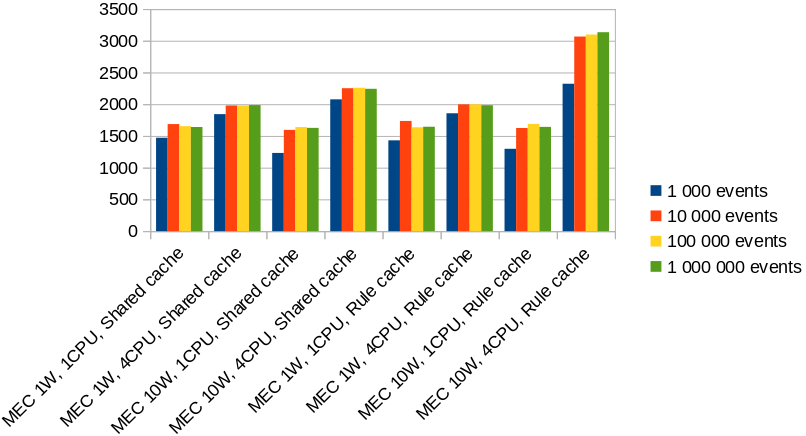
\includegraphics[scale=0.525]{figures/new-rule-format/performance-2.png}
\\
In the above graph, we see a drastic fall in events processed per second, because of the need to iterate over more rules. As expected, we see that rule-cache with 10W and 4CPU gives a 39.77\% increase compared against 10W, 4CPU and shared locking.

What is interesting here is the little difference between (1W, 1CPU), (10W, 1CPU), (1W, 4CPU) and the two different locking implementations. This makes sense, as the low amount of workers don't take advantage of the rule-based context locking, and will then fall to the same speed as shared context locking.

\subsubsection{Low signal, high noise dataset}
\todo{This experiment requires a bit more care. We should discuss context locking method, rules used and why we chose this dataset.}


What happens when we have a low signal, high noise dataset? We can see the result in Figure \cref{fig:comparing-lshn-hsln}. The following experiment explores that. Our hypothesis is that with a dataset where a single rule is triggered only once, we will see a drastic improvement over our high signal, low noise dataset. The reasoning behind this, is that if the events processed do not trigger any of our rules, we can process events much quicker. In addition, if the event does not trigger our rule, the context engine will not come in to play, and we will not have to do any sorts of locking.

This test has been run with a single rule and shared context locking. \n{Discuss why we chose this lock? Should we perhaps try the other as well?}

\begin{figure}[ht]
\centering
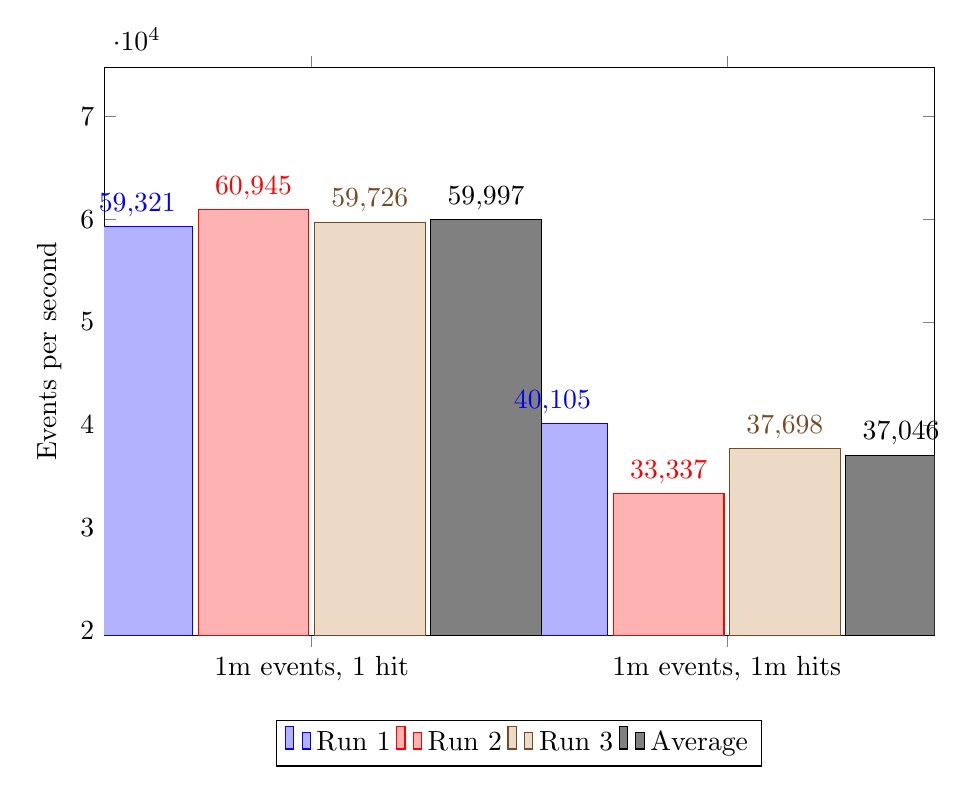
\begin{tikzpicture}
\begin{axis}[
    xtick=data,
	height=250pt,
	ylabel=Events per second,
	enlargelimits=0.5,
	legend style={at={(0.5,-0.15)},
	anchor=north,legend columns=-1},
	ybar,
	bar width=40pt,
	symbolic x coords={{1m events, 1 hit}, {1m events, 1m hits}},
	nodes near coords,
	nodes near coords style={above}
]
\addplot coordinates {({1m events, 1 hit},59321) ({1m events, 1m hits},40105)};
\addplot coordinates {({1m events, 1 hit},60945) ({1m events, 1m hits},33337)};
\addplot coordinates {({1m events, 1 hit},59726) ({1m events, 1m hits},37698)};
\addplot coordinates {({1m events, 1 hit},59997) ({1m events, 1m hits},37046)}; 
\legend{Run 1, Run 2, Run 3, Average}
\end{axis}
\end{tikzpicture}
\caption{Comparing low signal high noise with high signal low noise datasets }
\label{fig:comparing-lshn-hsln}
\end{figure}

\chapter{Discussion}
\label{chap:discussion}

In this chapter, we will discuss the results of our experiments, and how they line up with our research questions posed in \cref{chap:introduction}. We will also outline any future work.
This chapter provides a discussion of what implications the results of the experiments has, and presents different aspects of the work conducted.


The first question regarding the state of the art in event correlation has been addressed in Chapter \cref{chap:background} where we have highlighted relevant studies and options for doing event correlation. We highlighted several different methods for doing event correlation.

% How can we improve the way real time event correlation is done for Windows Event Logs
We have considered multiple ways that we can improve 

We reimplemented what we considered the most important parts of \acrshort{SEC} in Go, taking advantage of Go being a compiled program. As seen in \n{REF}, this showed a great increase in the event throughput of the system. As discussed, we added concurrency and threading, which allowed us to utilize the full capacity of the processor. As seen in  \n{REF}, this lead to a even greater event throghput.

We also implemented a new way to pre-handle event logs when ingesting. We called this tokenizing,  \n{REF} and along with using Sigma \n{REF} as a new rule format, we were able to increase the throughput even further, as seen by  \n{REF}.

As outlined in experiments  \n{REF}, we identified two different ways to do context locking, and showed that for larger datasets, using the rule-based context mutex gave some increase in the event throughput  \n{REF}.

This shows that we were not only able to improve the way real time event correlation is done for Windows Event Logs, but also show that our improvements give significant performance benefits.

First of all we will extrapolate some numbers from the Mordor datasets. As discussed in \cref{sec:dataset-analysiss}, the second scenario had an average events per 10 seconds of 678. This gives us 67.8 events per second. If we consider that the dataset contained 8 users and 5 hosts, we can try to make some assumptions regarding real world environments. If we consider an environment with 100 hosts, that would give us a ballpark estimation of 1356 events per second. If we consider an environment with 500 hosts, that brings our estimation to 6780 events per second. This is not taking into account any peaks in the data. If we consider the highest peak in the first scenario, as seen in \cref{fig:10-sec-day-1}. Given a network size of 500 hosts, that would give us a peak at about 22 800 events per second. Now, that is probably unrealistic, as not all the hosts in the network would peak at the same time, producing massive amount of logs.

\iffalse
What if we use more rules?

\fi

\iffalse
Interpretations: what do the results mean?
Implications: why do the results matter?
Limitations: what can’t the results tell us?
Recommendations: what practical actions or scientific studies should follow?
\fi


\section{Research questions}
...\\
The research presented in this thesis aims at improving real time event correlation...


The experiments conducted in this thesis evaluated a subset of possible features that might improve the performance of real time event correlation.
We chose to compare our solution against \acrshort{sec}, as that seems to be the most popular open-source software for rule-based event correlation and used in a wide variety of sectors. 

First of all we implemented a new solution that used the same rulesets at \acrshort{sec}, but implemented it using the compiled language Go. Running this using equal conditions like the same dataset, and only a single core, we were able to outperform SEC with 20-40\% using the high signal low noise dataset, and up to 89-135\% when comparing with the baseline dataset. This clearly shows the benefits of utilizing a compiled language when performance is an important criteria.

We implemented a better time management system that extracts the UTC timestamp from the log, and uses that for the time-based correlation as opposed to SEC which uses the time of when SEC reads the log line from input. The difference here does not play a role processing-wise, as the timestamps in the datasets are set to a single point in time, which replicates how SEC works in our new solution. In a real world scenario this would not be the case, and we consider our solution to be a better implementation than the one used in SEC.

We implemented functionality to take full advantage of the system hardware by using all cores available to use. This gave us an even bigger increase in throughput compared to both SEC and our own implementation using only a single core. We saw performance improvements of 59-80\% comparing our multi-threaded version to our single core version using the high signal low noise dataset, and improvements of 33-68\% when using the baseline dataset.

Lastly we implemented some changes to our solution that would depend less on regular expressions. To do this, we did two major changes: First we rewrote parts of the ingestion to tokenize each log entry, then we rewrote the rule parser to use Sigma rules instead. The benefits of this was clear, as we saw an even bigger performance boost..\n{Add some numbers here pls}

\begin{itemize}
    \item We were able to beat SEC in performance by implementing it using a compiled language and utilizing threading
    \item We were further able to enhance the speed by utilizing tokenization of the logs and using different rules
\end{itemize}

\section{Limitations of the study}
\label{sec:limitations}
We did not implement a one-to-one copy of \acrshort{sec} as we did not consider that to be of importance. We chose those features that we considered valuable. In addition, we did not create full feature parity with Sigma, only the parts necessary.

\section{Future work}
\label{sec:futurework}


\begin{itemize}
    \item Modularity
    \item Broader log support
    \item Distributed/scaling
\end{itemize}

We consider broader log support to be fairly simple to implement in the future. In addition, we focused on Sysmon as a subset of Windows Event logs, and expanding the ability to ingest regular Windows Event log is already done, but was not considered relevant as part of this thesis.

Distributed scaling: What could it tell us? Even more performance, harder to implement. Shared context is very tricky.

\todo{What could be expanded further upon in the future?}
\todo{Are there any experiments that we could have done, but didn't have the time to do? What could they tell us that we already didn't know?}
Full feature-parity with Sigma? With SEC?
\chapter{Conclusion}
\label{chap:conclusion}

\iffalse
Minioppsummering, med fokus på konsekvenser, konkludere om du har besvart RQ.

Her skal det ikke introduseres noe nytt! Trekker sammen de viktige tingene til slutt.

Inneholder også future work, her kan du utdype litt, men ingenting "nytt" her.
\fi
The goals of this thesis was to outlined the state of the art in real time event correlation, and implemented a solution that improves the way real time event correlation can be done with regards to Windows Event log correlation. This solution builds upon existing solutions.. \n{elaborate}

First of all we did a deep dive into the state of the art and considered several relevant types of event correlation. Rule-based event correlation was chosen for SEVERAL REASONS \n{add some reasons}, and relevant opponents was identified. \n{elaborate}

A implementation was created that utilized the same rule-set as SEC. We implemented multi-threading which saw a great effect. \n{elaborate}

A new implementation was proposed that uses different rules for correlating events. Two different methods for context management was explored as part of this. \n{elaborate}

The experiments and the associated results present the event processing and correlation throughout which showed a varying level of increased performance, depending on the dataset and methods used for context management. The highest speed improvement seen was up to 135\%. \n{elaborate}

In conclusion, this thesis has outlined the state of the art in real time event correlation, and implemented a solution that improves the way real time event correlation can be done with regards to Windows Event log correlation.
Different implementations have been created and tested for performance through experiments using datasets that are both realistic, and optimized for testing performance. The experiments served as proof-of-concept that we were able to enhance and improve the event processing throughput and correctness compared to existing solutions. As a result, this thesis has made a contribution to event correlation, and more specifically for correlating Windows Event logs in near real time.

\chapter*{\bibname}
\printbibliography[heading=none]

\appendix
\chapter{Sysmon to Syslog Python script}
\label{appendix:sysmon-to-syslog-python-script}

\lstinputlisting[
    caption={Sysmon to Syslog Python script},
    label=lst:pythonfile,
    language=Python
]{listings/sysmon-to-syslog.py}
\chapter{Extracting events in 10s intervals}
\label{appendix:extract-events-in-10s-intervals}

\lstinputlisting[
    caption={Extracting events in 10s intervals},
    label=lst:pythonfile,
    language=Python
]{listings/time.py}
\chapter{Extracting users from dataset}
\label{appendix:extract-users-from-dataset}

\lstinputlisting[
    caption={Extracting users from dataset},
    label=lst:extract-users-from-dataset,
    language=Python
]{listings/users.py}
\chapter{Extracting computers from dataset}
\label{appendix:extract-computers-from-dataset}

\lstinputlisting[
    caption={Extracting computers from dataset},
    label=lst:pythonfile,
    language=Python
]{listings/computers.py}
\chapter{SEC rule used in testing}
\label{appendix:sec-rule}

\lstinputlisting[
    caption={SEC rule used in testing},
    label=lst:sec-rule,
    language=Python
]{listings/windows.sec}
\chapter{Sigma rule used in testing}
\label{appendix:sigma-rule}

\lstinputlisting[
    caption={Sigma rule used in testing},
    label=lst:sigma-rule,
    language=Python
]{listings/sigma.yml}

\end{document}
